\documentclass[a4paper,twoside,12pt]{book}


% necessary packages
\usepackage[T1]{fontenc}    % kódování písma
\usepackage[nottoc]{tocbibind}      % citace
\usepackage[utf8]{inputenc}     % vstupní znaková sada tohoto dokumentu: UTF-8
\usepackage{makecell}

\usepackage[resetfonts]{cmap}
\usepackage{lmodern}
\usepackage{xargs}
\usepackage[title]{appendix}
\usepackage{import}
\usepackage[a4paper, hmarginratio=3:2]{geometry} % využití A4 stránky a nastavení okrajů (u vazby bude širší)
\usepackage{upgreek}
\usepackage{pdfpages} % pokud nemáte formulář "Zadání bak./dipl. práce" naskenovaný jako PDF, tak ZAKOMENTUJTE
\usepackage[hidelinks,unicode]{hyperref} % v PDF budou klikací odkazy ("hidelinks" je nebude rámovat)
\usepackage{emptypage}
\usepackage{graphicx} % balíček pro vkládání rastrových grafických souborů (PNG apod.)
%\usepackage{epsfig} % balíčky pro vkládání grafických souborů typu EPS
\usepackage{float} % rozšířené možnosti umístění obrázků

\usepackage[font=small,labelfont=bf]{caption}
%\usepackage{caption} % pro popisky obrázků, tabulek atd.

\usepackage{tabularx} % rozšířené možnosti tabulek

\usepackage{listings}  % balíček vhodný pro ukázky zdrojového kódu v~textu práce/příloh. Nutno nastavit! http://ftp.cvut.cz/tex-archive/macros/latex/contrib/listings/listings.pdf
\usepackage{amsmath} % balíček pro pokročilou matematickou sazbu
\usepackage{amssymb}
%\usepackage{color} % pro možnost barevného textu
%\usepackage{fancybox} % umožňuje pokročilé rámečkování
%\usepackage{minipage}
%\usepackage{index} % nutno použít v případě tvorby rejstříku balíčkem makeindex
%\newindex{default}{idx}{ind}{Rejstřík} % zavádí rejstřík v případě použití balíku index
\usepackage{tocloft}
\usepackage{paralist}

% Proper bibliography
\usepackage[style=iso-numeric, backend=biber, language=czech]{biblatex}
\usepackage{csquotes}
\usepackage{amsthm}
\addbibresource{ref.bib}


\theoremstyle{definition}
\newtheorem{define}{Definice}[section]

%% nice header style
\usepackage{fancyhdr}

%% elements, isotopes,...
\usepackage[version=3]{mhchem}

\usepackage{gensymb}

\usepackage[printonlyused,footnote]{acronym}

%%% Specification of all necessary stuff %%%
% ========================================


% Specification of the author and consultants
\newcommand{\autor}{A. Nikolov, J. Sobotka, R. Šimeček, J. Zejda}   

% Specification of thesis -- copy and paste from your task list
\newcommand{\nazevcz}{Měření úniků mobilního spoje}

\newcommand{\rok}{2023}  % rok odevzdání práce (jen rok odevzdání, nikoli celý akademický rok!)
\newcommand{\skola}{\cvut}
\newcommand{\fakulta}{\fel}
\newcommand{\katedra}{Katedra elektromagnetického pole}
\newcommand{\kde}{Praze} % studenti z Děčína ZMĚNÍ na: "Děčíně" (doplní se k "prohlášení")
\newcommand{\program}{Elektronika a komunikace} % změňte, pokud máte jiný stud. program

%% LANGUAGE SETTINGS
% Uncomment exactly one block

%==================
%% CZECH
\usepackage[czech]{babel} % česky psaná práce, typografická pravidla. Překládejte pomocí "latex.exe" nebo "pdflatex.exe"

% Uncomment exactly one 
\newcommand{\druh}{Semestrální projekt II} 
%\newcommand{\druh}{Výzkumný úkol} 
%\newcommand{\druh}{Diplomová práce}

% Intendation
\usepackage{indentfirst}
\newcommand{\stdindent}{\setlength{\parindent}{2em}}
\newcommand{\stdskip}{\setlength{\parskip}{0em}}
%==================

%==================
%% SLOVAK
% \usepackage[slovak]{babel} 
%==================


%==================
%% ENGLISH
% \usepackage[english]{babel}

% Uncomment exactly one 
%\newcommand{\druh}{Bachelor thesis} 
%\newcommand{\druh}{Research project} 
%\newcommand{\druh}{Master thesis}

% Intendation
% \newcommand{\stdindent}{\setlength{\parindent}{0em}}
% \newcommand{\stdskip}{\setlength{\parskip}{1em}}
%==================



% Insert scan of your task -- put it in "img" folder -- 2 separate PDFs recommended
\newcommand{\skenZadaniPredni}{specimen1.pdf}
\newcommand{\skenZadaniZadni}{specimen2.pdf}

% Keywords in zde NAPIŠTE česky max. 5 klíčových slov AND translate them into english
\newcommand{\klicova}{slovo1, slovo2, slovo3}  
\newcommand{\keyword}{keyword1, keyword2, keyword3}
\newcommand{\abstrCZ}{% zde NAPIŠTE abstrakt v češtině (cca 7 vět, min. 80 slov)
Tato práce se zabývá psaním závěrečných prací.
}
\newcommand{\abstrEN}{% zde NAPIŠTE abstrakt v angličtině
The thesis deals with the issue of thesis writing. 
}
\newcommand{\prohlaseni}{% text prohlášení můžete mírně upravit
Prohlašuji, že jsem svou bakalářskou práci vypracoval\woman{} samostatně a použil\woman{} jsem pouze podklady (literaturu, projekty, SW atd.) uvedené v přiloženém seznamu.
} 
\newcommand{\podekovani}{%Podekovani se doporucuje neprehanet
 Děkuji Ing. Eleonoře Krtečkové, Ph.D. za vedení mé bakalářské práce a za podnětné návrhy, které ji obohatily.
% NEBO:
% Děkuji vedoucímu práce doc. Pafnutijovi Snědldítětikaši, Ph.D. za neocenitelné rady a pomoc při tvorbě bakalářské práce.
}

% Page style -- uncomment exactly one
% 
% Style 1 -- fancy -- nice looking, but unfortunatelly, not debugged yet :(
\pagestyle{fancy}
\fancyfoot{}
\fancyhead[RO,LE]{\thepage}
\fancyhead[RE]{\nouppercase{\leftmark}}
\fancyhead[LO]{\nouppercase{\rightmark}}

% Style 2 -- plain
% \pagestyle{plain}      % stránky číslované dole uprostřed


% Page numbering
\pagenumbering{arabic} % číslování stránek arabskými číslicemi

% Depth of table of contents (ToC) (2 is RECOMMENDED, other are believed to be confusing and poorly arranged!
% 0 = only parts and chapters are included in ToC
% 1 = parts, chapters, sections
% 2 = parts, chapters, sections, subsections
% 3 = parts, chapters, sections, subsections, subsubsections
\setcounter{tocdepth}{2}


% Margins 
\topmargin=-10mm      % horní okraj trochu menší
\textwidth=150mm      % šířka textu na stránce
\textheight=250mm     % "výška" textu na stránce


% Font size
\renewcommand\cftchapfont{\small\bfseries}
\renewcommand\cftsecfont{\footnotesize}
\renewcommand\cftsubsecfont{\footnotesize}

\renewcommand\cftchappagefont{\small\bfseries}
\renewcommand\cftsecpagefont{\footnotesize}
\renewcommand\cftsubsecpagefont{\footnotesize}

% Spacing
\frenchspacing % za větou bude mezislovní mezera (v anglických textech je mezera za větou delší)
\widowpenalty=1000 % "síla" zákazu vdov (= jeden řádek ze začátku odstavce na konci stránky)
\clubpenalty=1000 % "síla" zákazu sirotků (= jeden řádek/slovo z konce odstavce samostatně na začátku stránky)
\brokenpenalty=1000 % "síla" zákazu zlomu stránky za řádkem, který má na konci rozdělené slovo

% ==== Aliases, own commands ====


% Aliases
\newcommand{\ti}{\textit} % zkrácený příkaz pro kurzívu
\newcommand{\tb}{\textbf} % zkrácený příkaz pro tučné písmo
\newcommand{\bv}{\mathbf} % zkrácený příkaz pro tučné vektory v math mode

% Smaller lists

% Compact itemize
\newcommandx{\cit}[1]{
        \begin{compactitem}
                #1
        \end{compactitem}
}

% Compact enumerate
\newcommandx{\cen}[1]{
        \begin{compactenum}
                #1
        \end{compactenum}
}


% Faster and better images

% Single figure
\newcommandx{\pic}[5][4=0.8,5=H]{%
\begin{figure}[#5]
\centering
\includegraphics[width=#4\textwidth]{./img/#1}
\caption[#2]{#3}
\label{#1}
\end{figure}
}

% Two pictures side-by-side
\newcommandx{\dpic}[9][7=0.49,8=0.98,9=H]{%
\begin{figure}[#9]
    \centering
    \begin{minipage}{#7\textwidth}
        \centering
        \includegraphics[width=#8\textwidth]{img/#1} % first figure itself
        \caption[#3]{#4}
        \label{#1}
    \end{minipage}\hfill
    \begin{minipage}{#7\textwidth}
        \centering
        \includegraphics[width=#8\textwidth]{img/#2} % second figure itself
        \caption[#5]{#6}
        \label{#2}
    \end{minipage}
\end{figure}
}

% Three figures side-by-side... Not really sure, whether it looks good
\newcommandx{\tpic}[9]{%
\begin{figure}[H]
    \centering
    \begin{minipage}{0.3\textwidth}
        \centering
        \includegraphics[width=0.95\textwidth]{img/#1} % first figure itself
        \caption[#2]{#3}
        \label{#1}
    \end{minipage}\hfill
    \begin{minipage}{0.3\textwidth}
        \centering
        \includegraphics[width=0.95\textwidth]{img/#4} % second figure itself
        \caption[#5]{#6}
        \label{#4}
    \end{minipage}\hfill
    \begin{minipage}{0.3\textwidth}
        \centering
        \includegraphics[width=0.95\textwidth]{img/#7} % second figure itself
        \caption[#8]{#9}
        \label{#7}
    \end{minipage}
\end{figure}
}

% Better footnotes above punctuation
\newcommand{\footnotei}[2]{%
\mbox{%
\setbox0\hbox{#1}%
\copy0%
\hspace{-\wd0}}%
\footnote{#2}%
}

% Equations
\newcommandx{\eq}[1]{
        \begin{equation}
                #1
        \end{equation}
}
\newcommandx{\eqa}[1]{
        \begin{align}
                #1
        \end{align}
}

% Units
\newcommand{\jdt}[1]{
        $\mathrm{#1}$
}
        
\newcommand{\jde}[1]{
        \mathrm{#1}
}

% Derivative faster
\newcommand{\der}[2]{
        \frac{\mathrm{d} #1}{\mathrm{d} #2}
}

% N-th derivative faster
\newcommand{\nder}[3]{
        \frac{\mathrm{d}^{#3} #1}{\mathrm{d} {#2}^{#3}}
}

% Partial derivative faster
\newcommand{\pder}[2]{
        \frac{\partial #1}{\partial #2}
}

% N-th partial derivative faster
\newcommand{\npder}[3]{
        \frac{\partial^{#3} #1}{\partial {#2}^{#3}}
}

% Auto-sized brackets

\renewcommand{\(}{
        \left(
}
\renewcommand{\)}{
        \right)
}

\renewcommand{\[}{
        \left[
}
\renewcommand{\]}{
        \right]
}


% CTU stuff
\newcommand{\cvut}{České vysoké učení technické v~Praze}

% CTU Faculties
\newcommand{\fjfi}{Fakulta jaderná a fyzikálně inženýrská}
\newcommand{\fel}{Fakulta elektrotechnická}
\newcommand{\fit}{Fakulta informačních technologií}

% FNSPE 
\newcommand{\km}{Katedra matematiky}
\newcommand{\kf}{Katedra fyziky}
\newcommand{\kvhj}{Katedra humanitních věd a jazyků}
\newcommand{\kipl}{Katedra inženýrství pevných látek}
\newcommand{\kfe}{Katedra fyzikální elektroniky}
\newcommand{\kmat}{Katedra materiálů}
\newcommand{\kjch}{Katedra jaderné chemie}
\newcommand{\kdaiz}{Katedra dozimetrie a aplikace ionizujícího záření}
\newcommand{\kjr}{Katedra jaderných reaktorů}
\newcommand{\ksi}{Katedra softwarového inženýrství}
\newcommand{\di}{Dopplerův institut}

\newcommand{\logoCVUT}{
\includegraphics{img/symbol_cvut_konturova_verze_cb.pdf}} % logo ČVUT -- podle grafického manuálu ČVUT platného od prosince 2016. Pokud nevyhovuje PDF-verze, tak použijte jinou variantu loga: https://www.cvut.cz/logo-a-graficky-manual -> "Symbol a logo ČVUT v Praze"). Pokud chcete logo úplně vynechat, zadejte místo "\includegraphics{...}" text "\vspace{35mm}"


\renewcommand{\sectionautorefname}{v sekci}

\bibliography{ref}
\begin{document}

\frontmatter

\thispagestyle{empty}

\begin{center}
	{\LARGE
		\skola\par
		\fakulta
	}
    \vspace{10mm}

    \begin{tabular}{c}
		\tb{\katedra} \\[3pt]   
    \end{tabular}

   \vspace{10mm} \logoCVUT \vspace{15mm} 

   {\huge \tb{\nazevcz}\par}
   \vspace{5mm}   
   {\huge \tb{\nazeven}\par}
   
   \vspace{15mm}
   {\Large \MakeUppercase{\druh}}

   \vfill
   {\large
    \begin{tabular}{ll}
    Vypracovali: & \autor\\
    Rok: & \rok
    \end{tabular}
   }
\end{center}

\clearpage{\pagestyle{empty}\cleardoublepage} % prázdná stránka za tou "titulní", bez čísla

\newpage  % SEM NESAHEJTE!
\thispagestyle{empty} % SEM NESAHEJTE!

\newpage % SEM NESAHEJTE!
\thispagestyle{empty}  % SEM NESAHEJTE!

\newpage  % SEM NESAHEJTE!
\parskip=0pt
\begin{small}
\tableofcontents % SEM NESAHEJTE!
\end{small}
\parskip=7pt
\newpage % SEM NESAHEJTE!


%--------------------------------------------------------
%|         Zde začíná SAMOTNÁ PRÁCE (text)              |
%--------------------------------------------------------
%%%%%%%%%%%%%%%%%%%%%%%%%%%%%%%%%%%%%%%%%%%%%%%%%%%%%%%%%%%
\listoffigures
\listoftables

\mainmatter

\stdindent
\stdskip

\chapter*{Úvod} % SEM NESAHEJTE!
\addcontentsline{toc}{chapter}{Úvod} % SEM NESAHEJTE!
\markboth{Úvod}{Úvod}
\section{Cíl projektu}
Cílem projektu je realizovat dva typy měření:

První měření se zabývá empirickým modelem. Jedna anténa je pevně umístěna na stojanu, zatímco druhá simuluje mobilní terminál. Cílem je získat závislost ztrát na poloze obou antén ve statickém prostředí pro úzkopásmový přenos. Nejjednodušší způsob je zaznamenávat úroveň při pohybu terminálu konstantní rychlostí po přímce směrem k/od pevné antény.

Druhé měření se zabývá měřením úniků způsobených vícecestným šířením. Obě antény jsou pevně umístěny na stojanech v dostatečné vzdálenosti (pro dané prostředí) na přímou viditelnost. Časový průběh přijímané úrovně úzkopásmového signálu je zaznamenán po dobu cca jedné minuty pro minimálně tři případy: v prvním neovlivňujte okolní prostředí (resp. spoj), ve druhém se naopak pokuste co nejvíce dynamicky spoj narušovat (např. pohybem členů týmu zastiňujícím přímou viditelnost mezi anténami) a ve třetím se pokuste dynamiku změn ještě zvýšit a zároveň dosáhnout trvalého zastínění spoje (za tím účelem můžete i změnit polohu antén). 


\section{Oficiální zadání}
\begin{enumerate}
\item Realizovat měření v terénu za účelem lepšího porozumění podstatě úniků mobilního spoje v pásmu UHF (300 MHz - 3 GHz) v různých prostředích. 
\item Využít měřená data pro odvození empirického modelu závislosti ztrát na vzdálenosti. 
\item Na základě výsledků měření statisticky analyzovat úniky způsobené vícecestným šířením. 
\end{enumerate}

\section{Použité vybavení}
Během měření bylo použito následující vybavení:
\begin{itemize}
    \item USB SDR Adalm Pluto pro vysílání, 
    \item Přenosný přijímač Rohde \& Schwarz PR100, 
    \item 2x všesměrová anténa se stojanem, 
    \item Mobilní telefon pro dokumentaci měření,
    \item Laserový dálkoměr Nikon Prostaff S 6x21 7.5
\end{itemize}

\begin{figure}[h!]
    \centering
    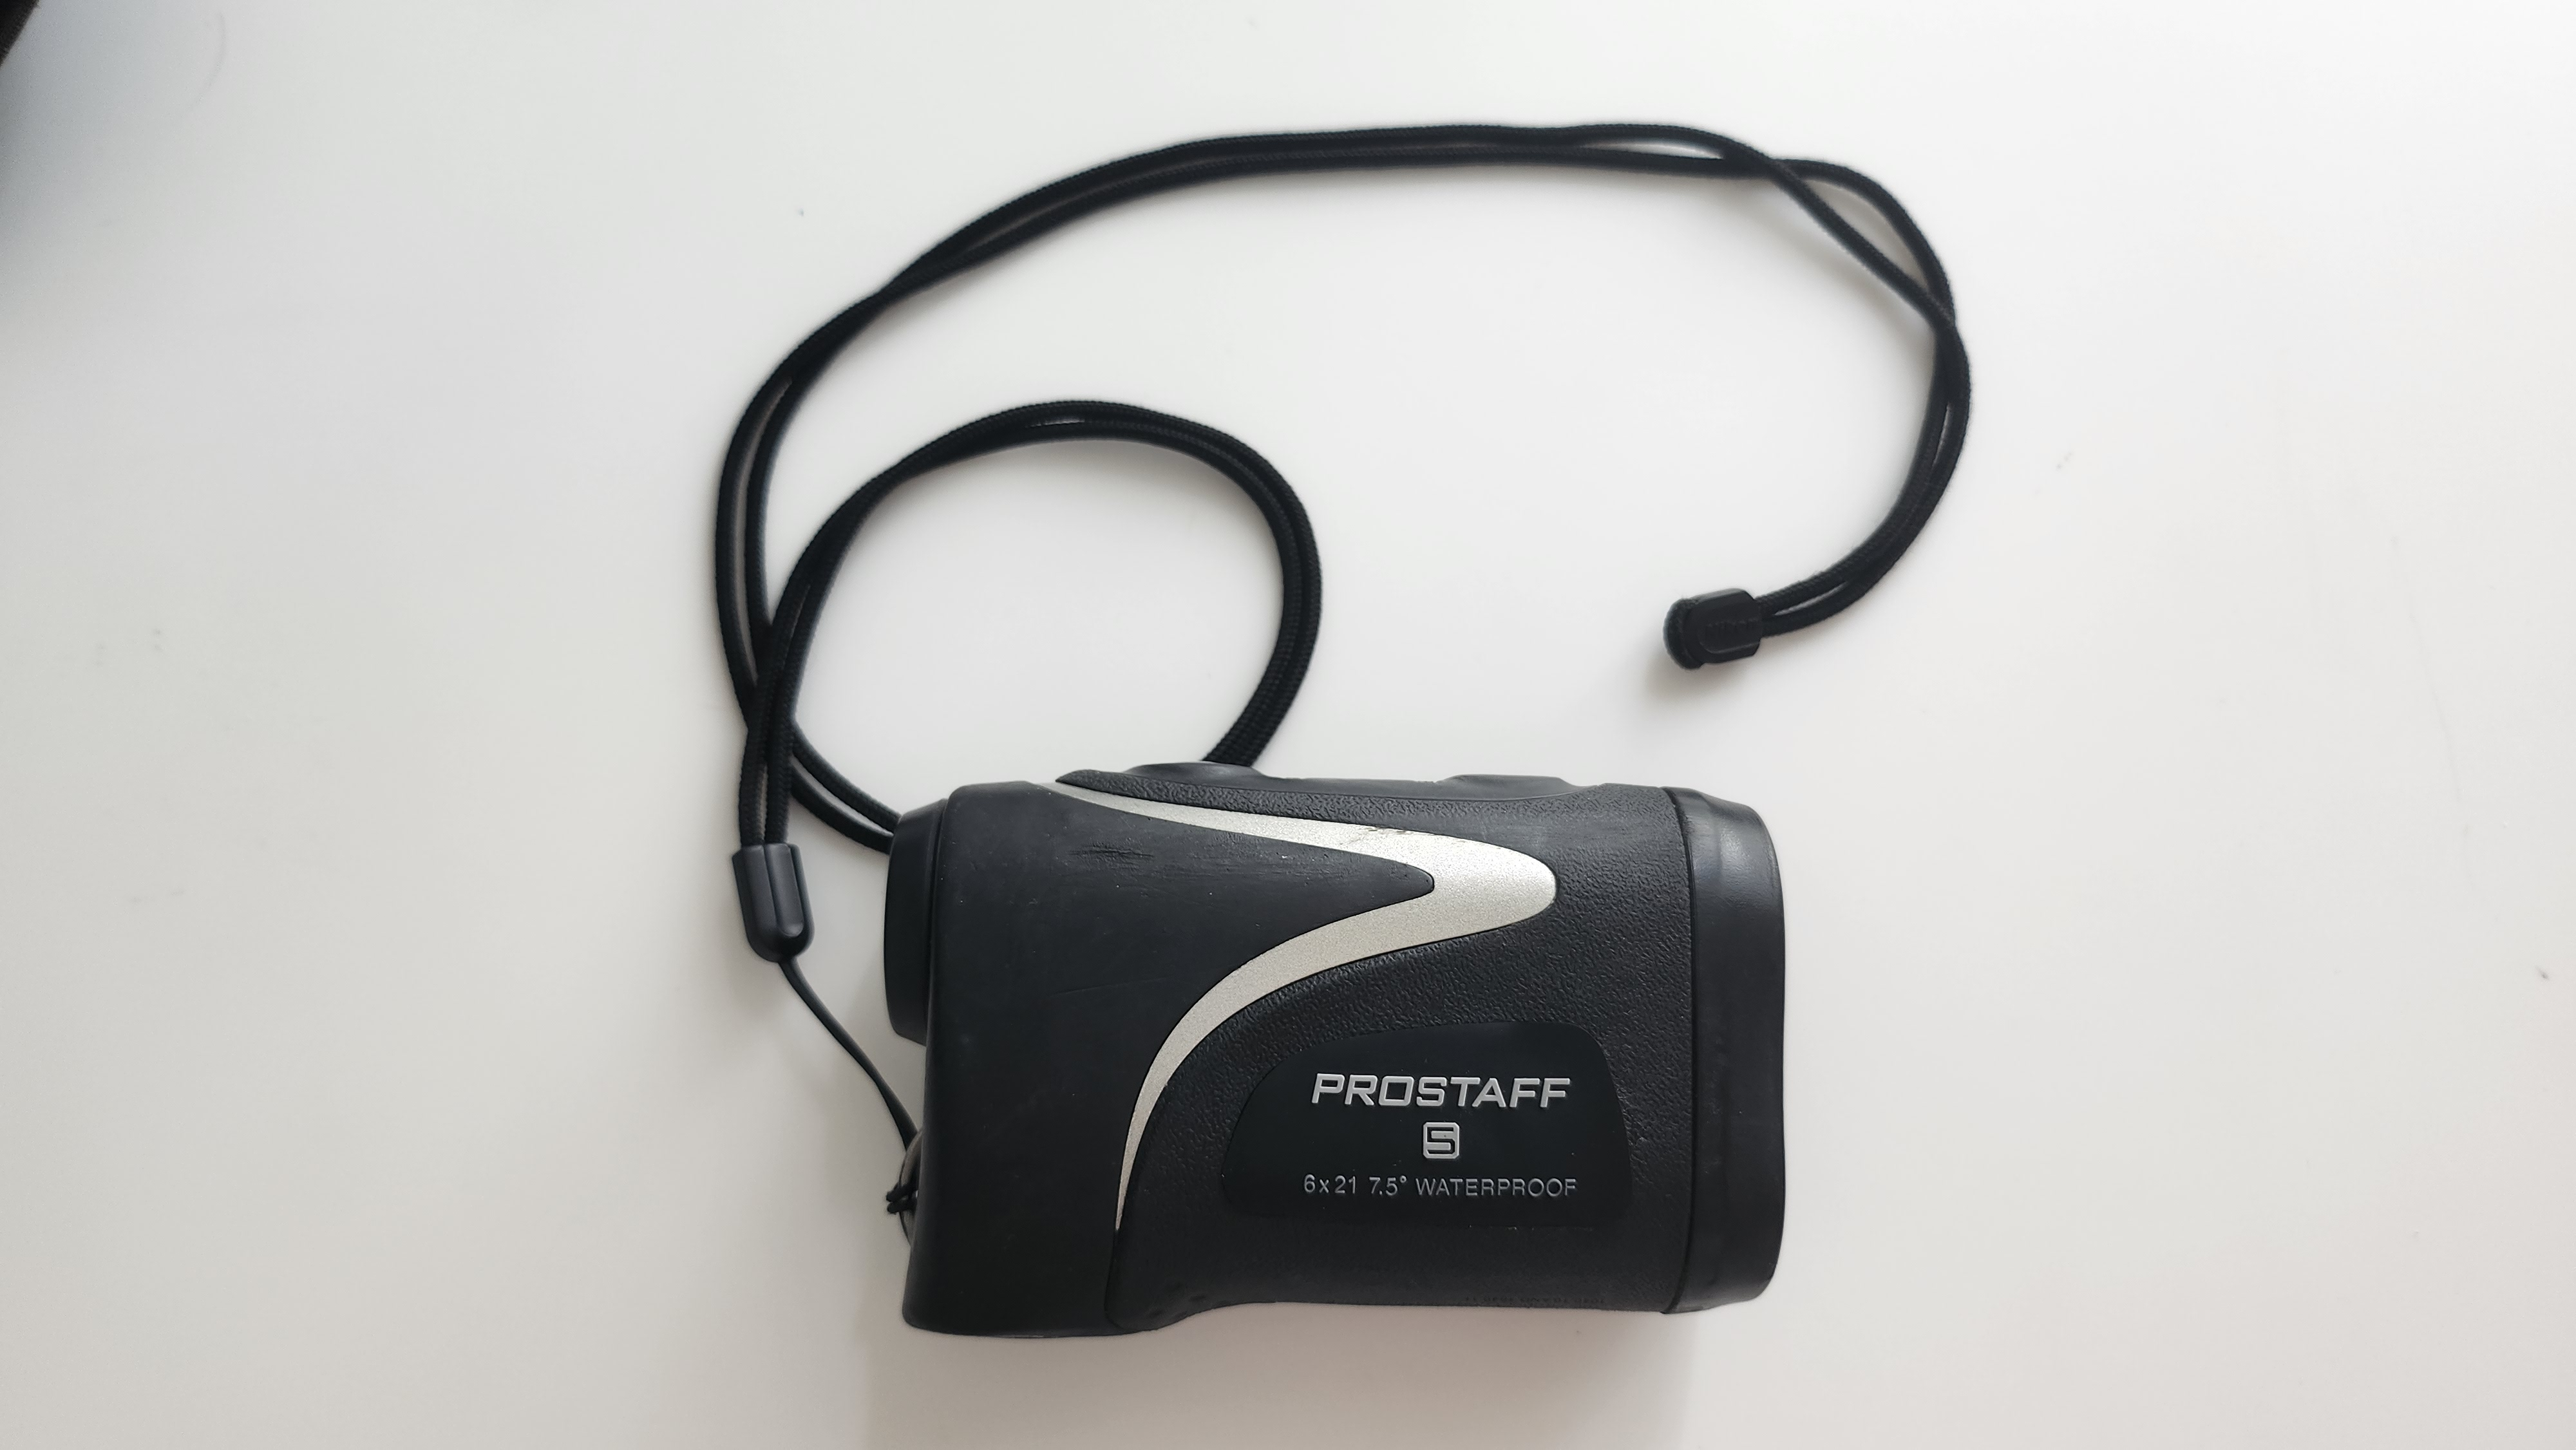
\includegraphics[scale=0.075]{img/dalkomer.jpg}
    \caption{Laserový dálkoměr Nikon Prostaff S 6x21 7.5}
    \label{fig:my_label}
\end{figure}

\begin{figure}[h!]
    \centering
    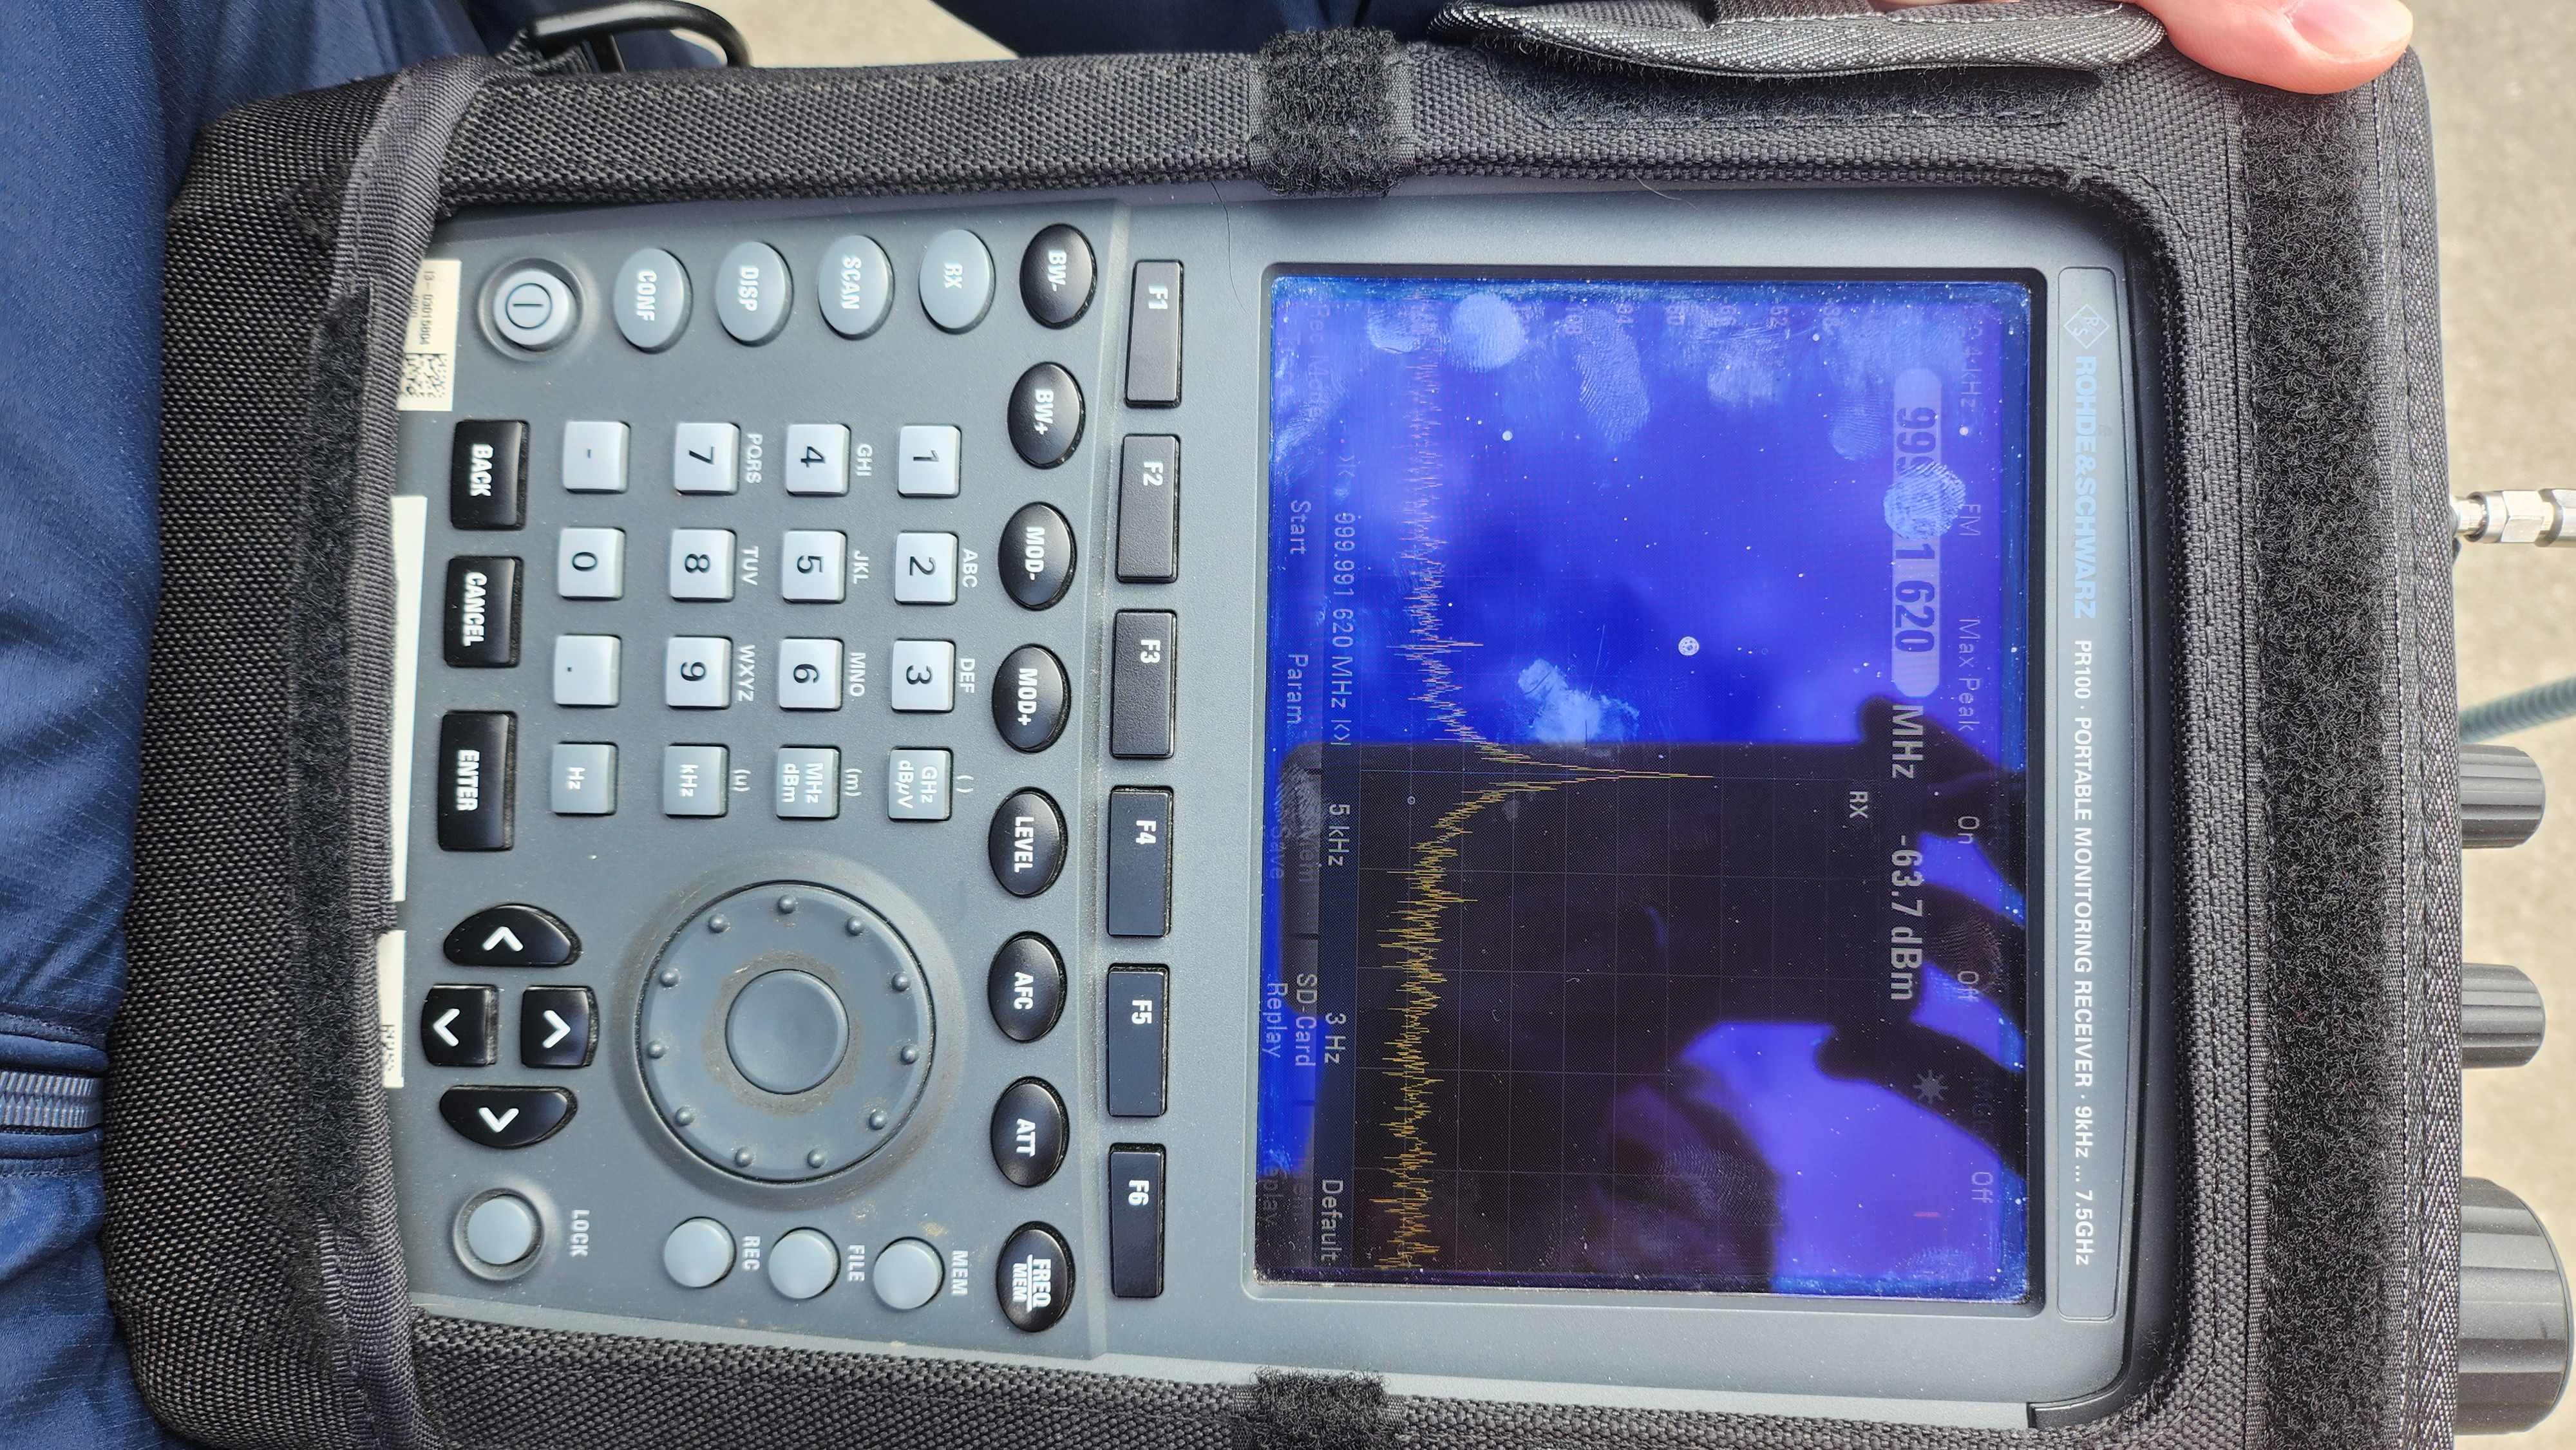
\includegraphics[angle=90,scale=0.06]{img/prijimac1.jpg}
    \caption{Přenosný přijímač Rohde \& Schwarz PR100 s krytem v terénu}
    \label{fig:my_label}
\end{figure}

\begin{figure}[h!]
    \centering
    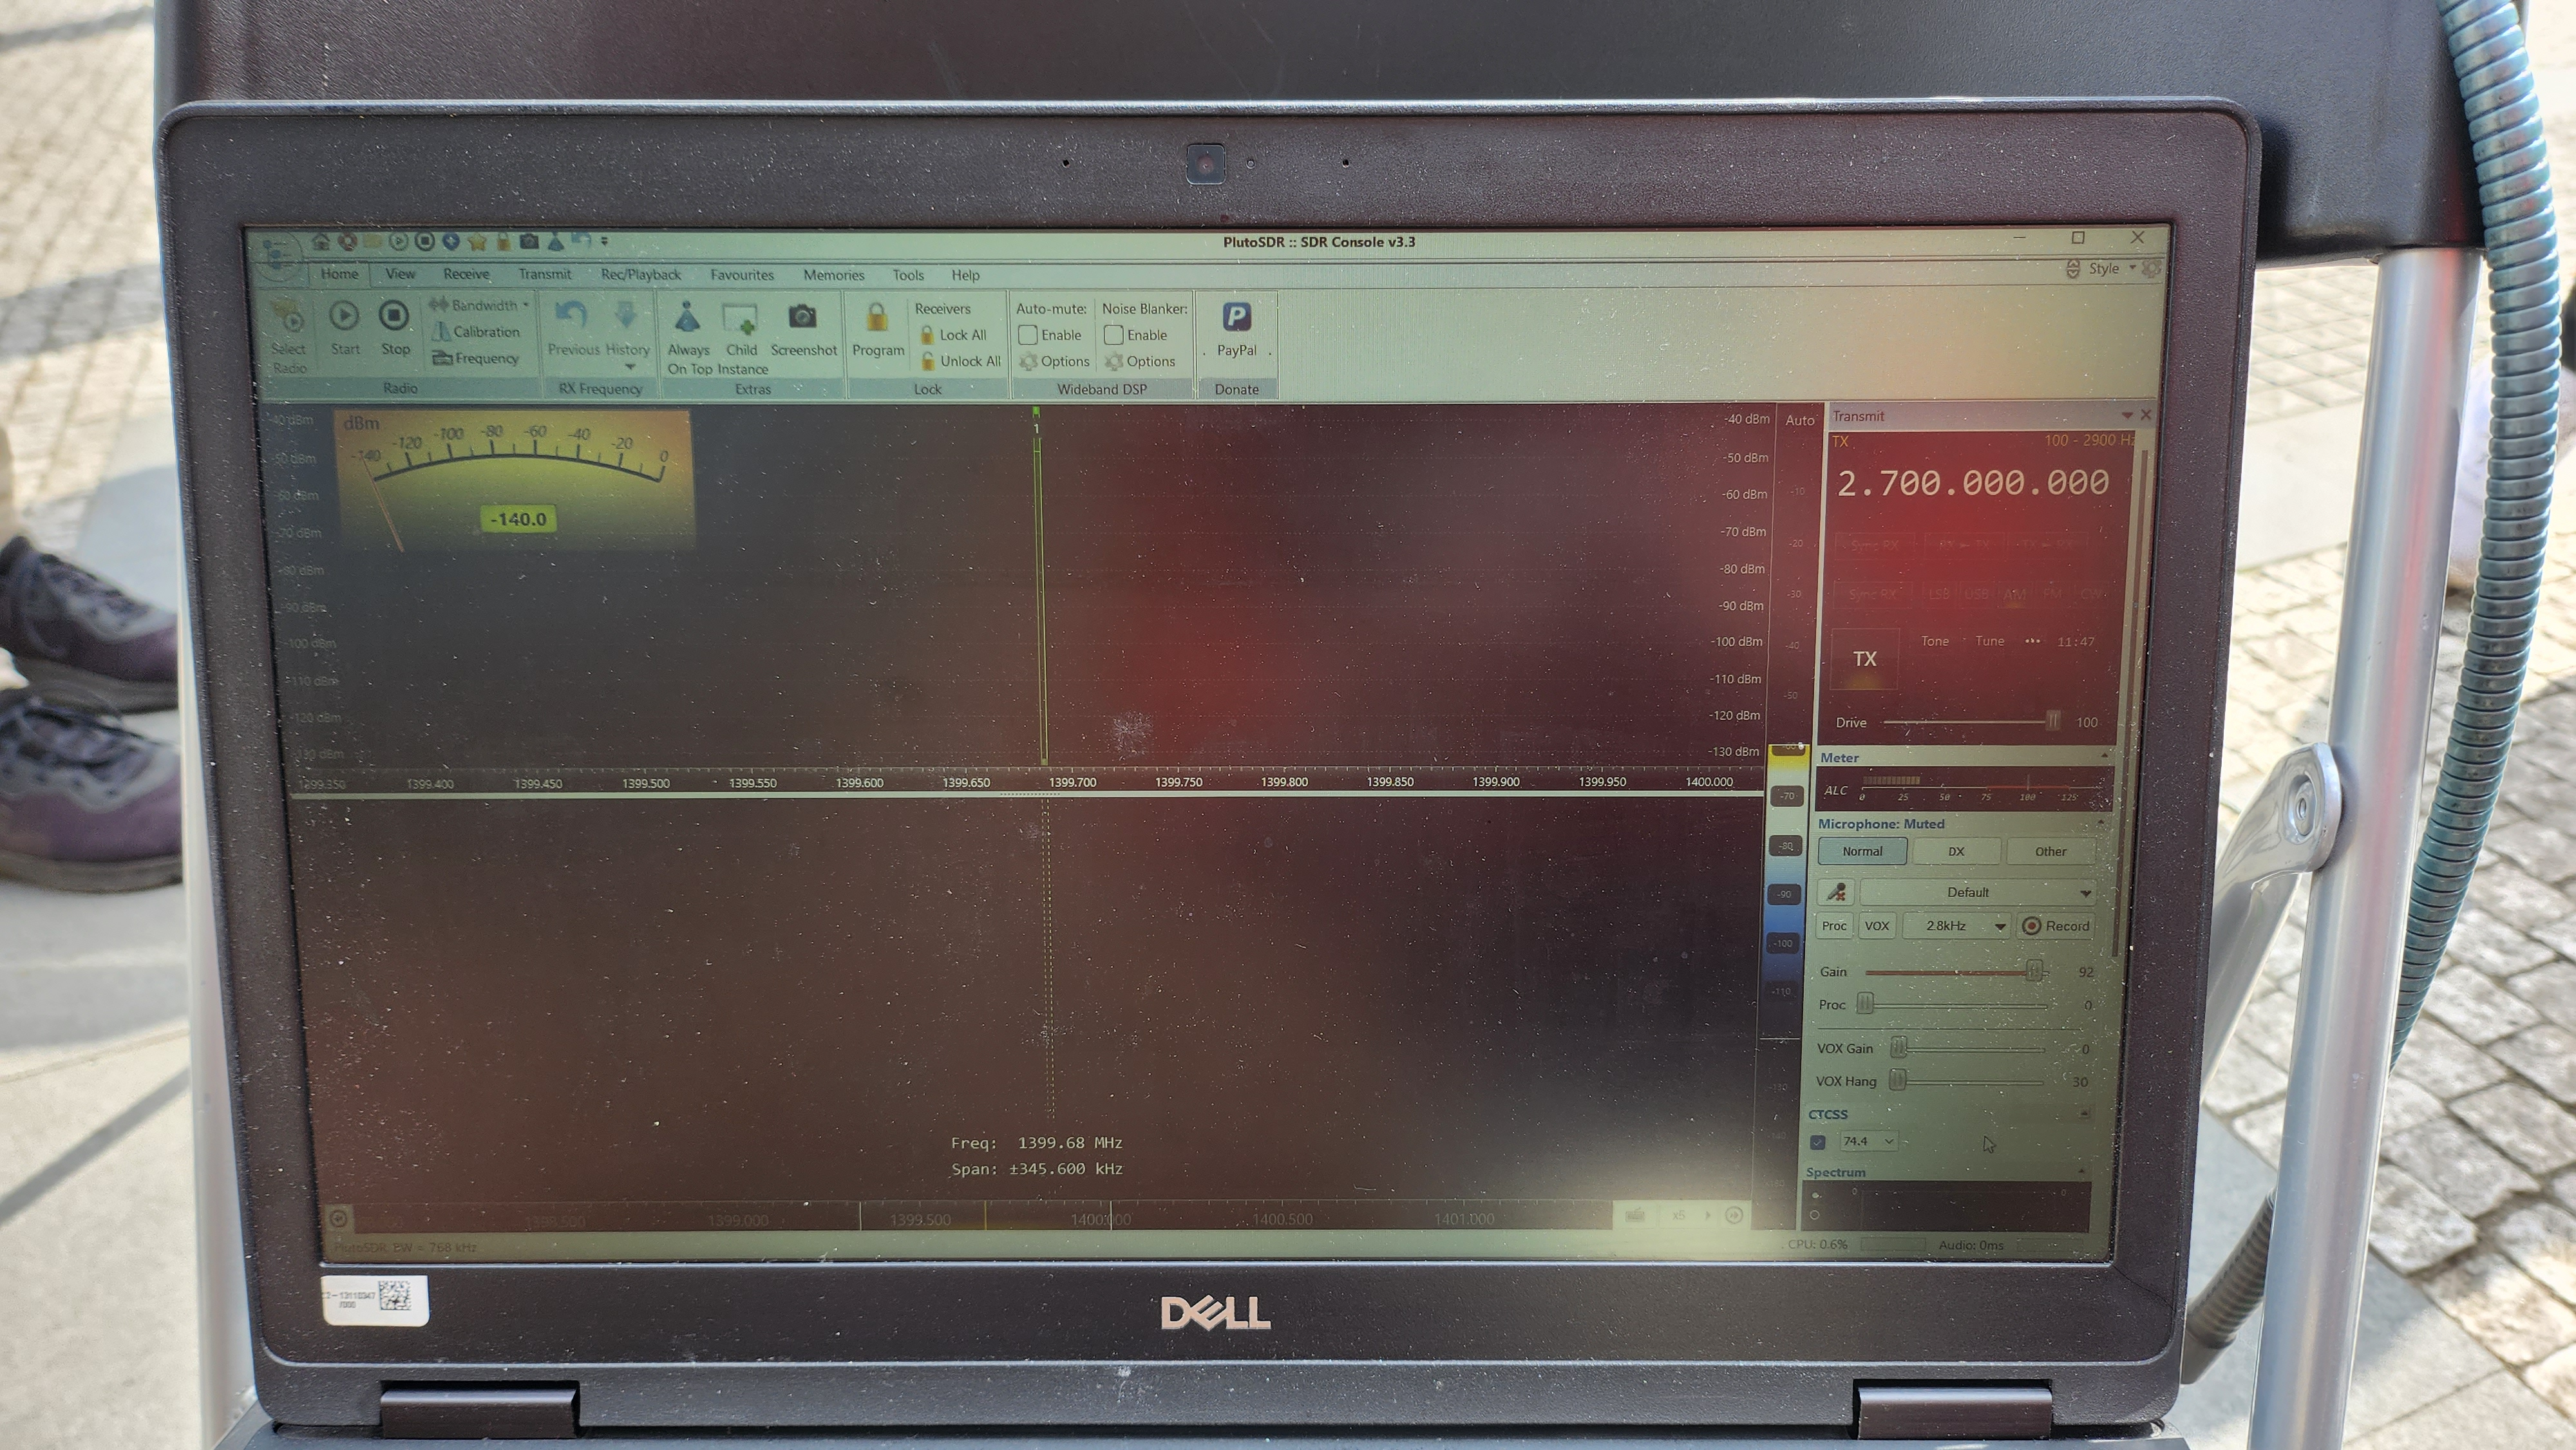
\includegraphics[scale=0.075]{img/notebook.jpg}
    \caption{Software pro vysílání běžící na notebooku v terénu}
    \label{fig:my_label}
\end{figure}

\begin{figure}[h!]
    \centering
    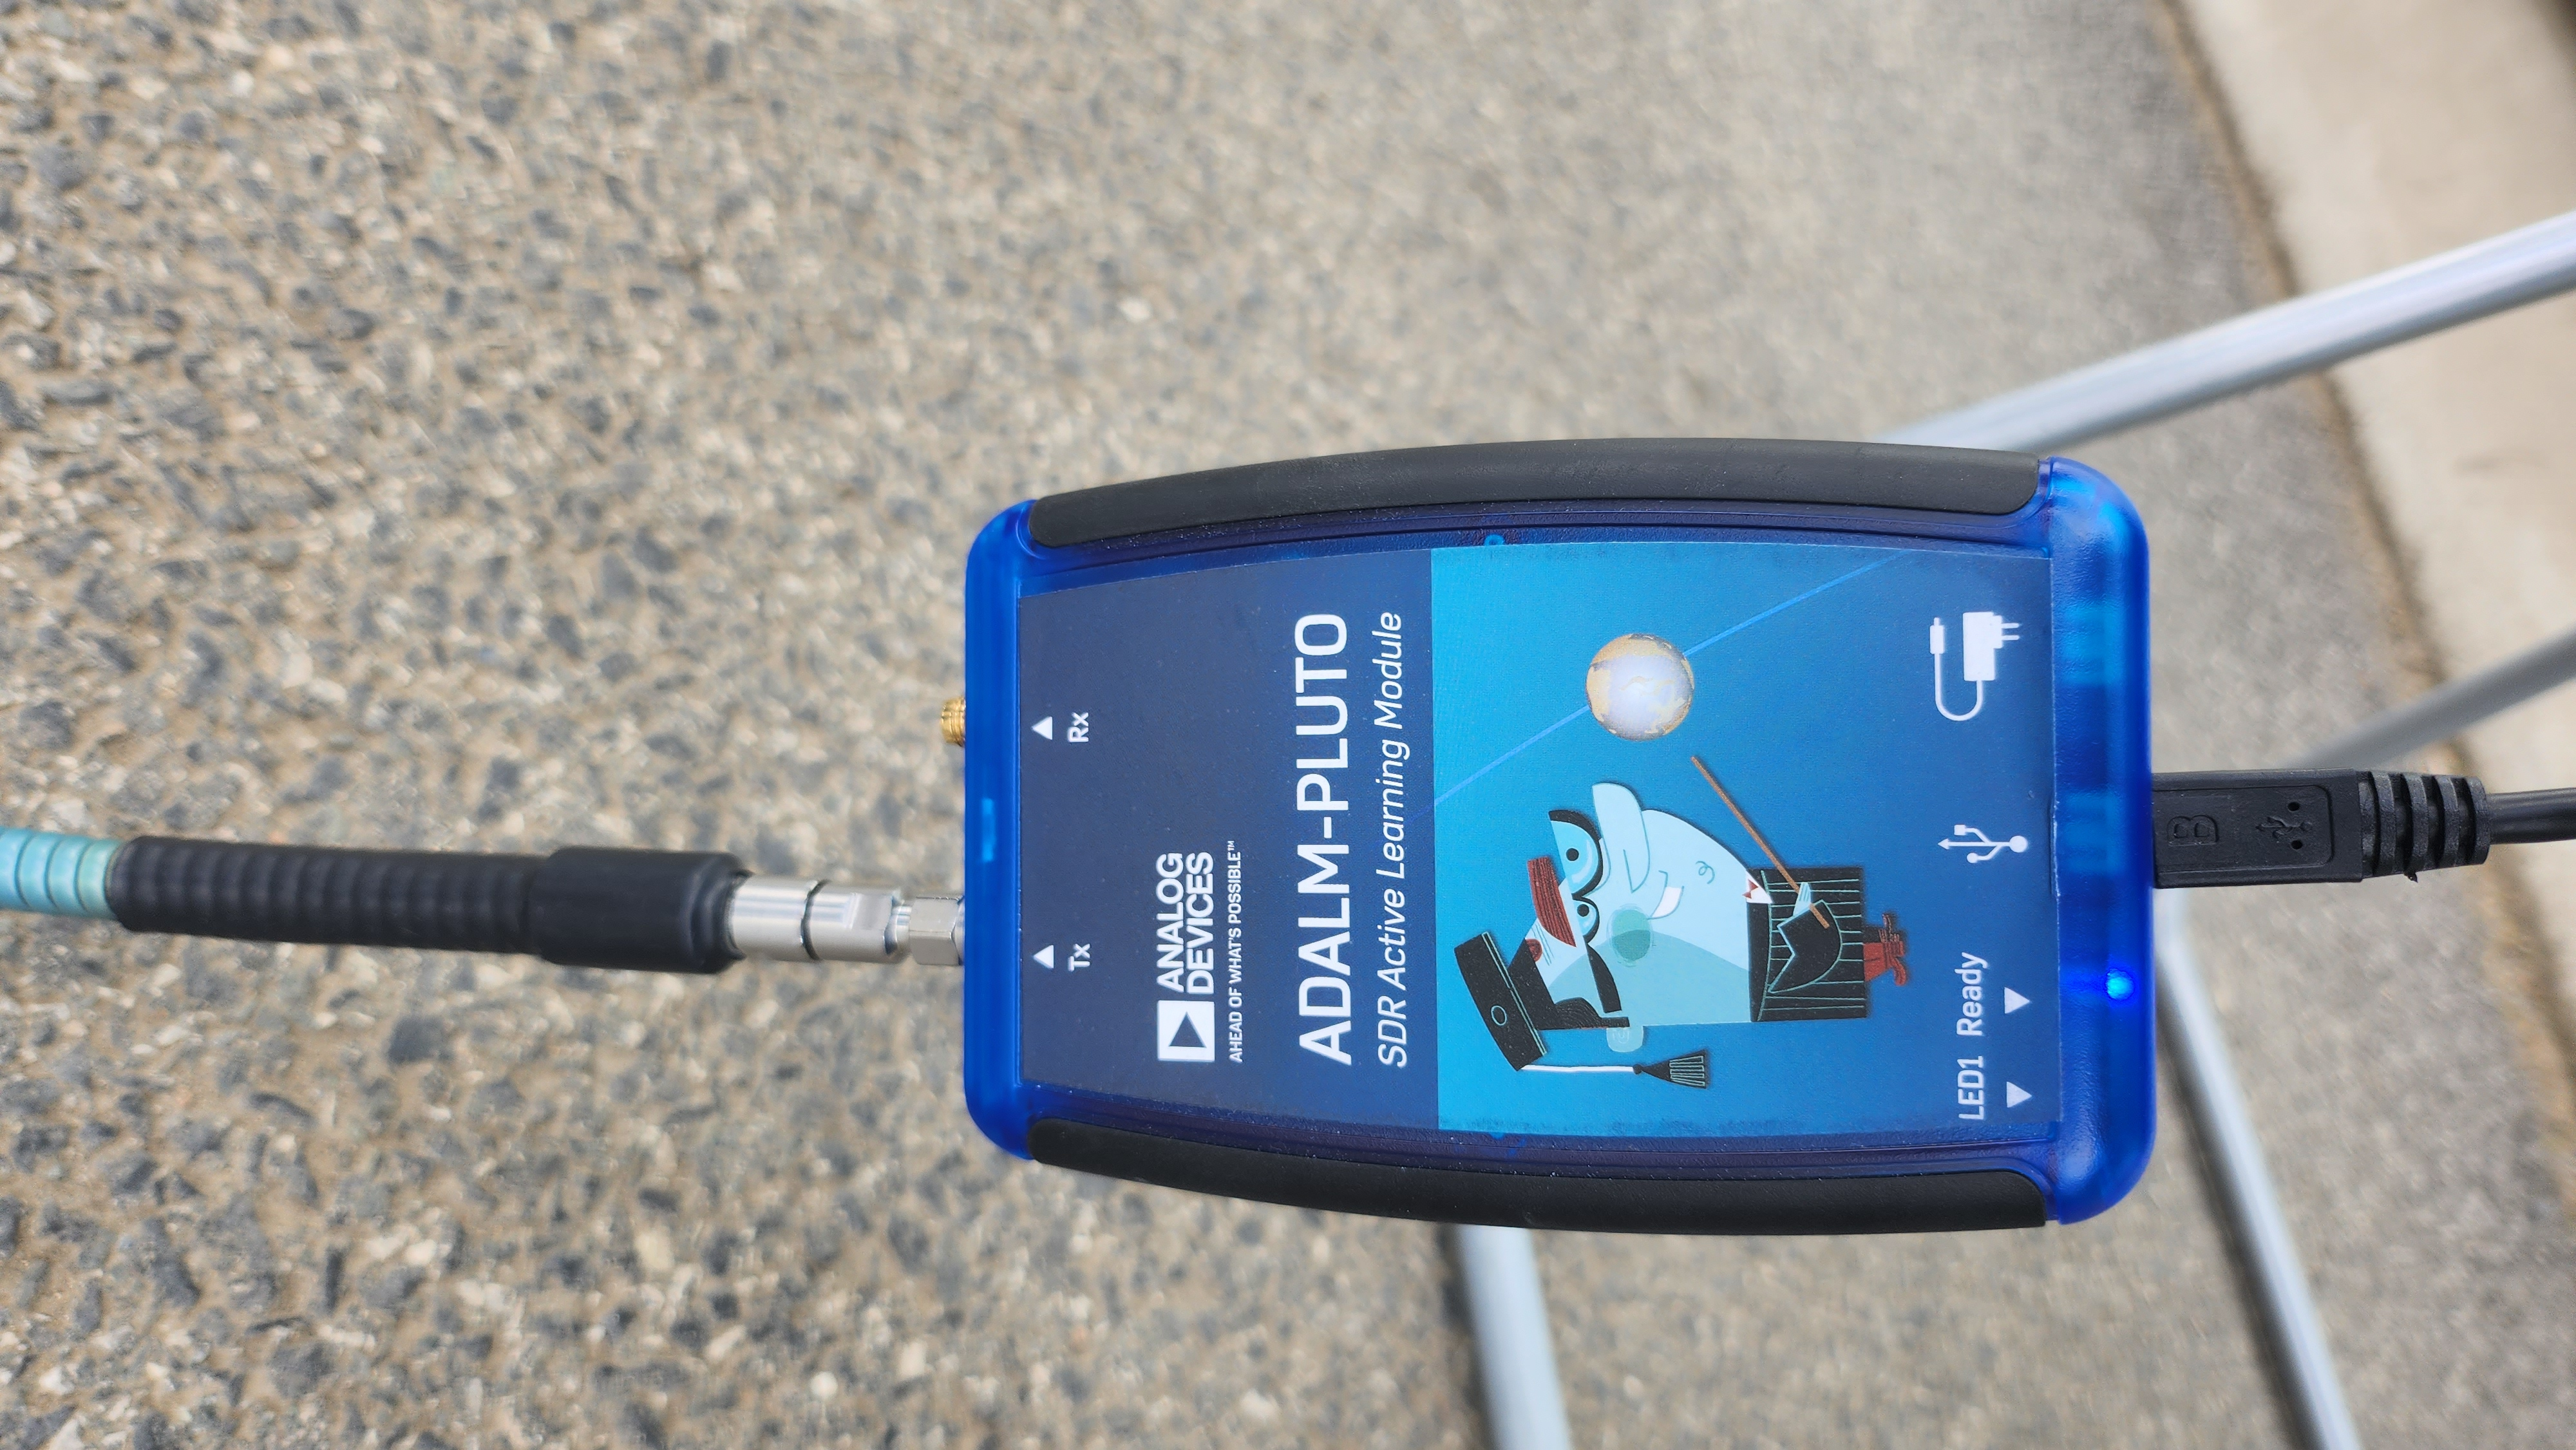
\includegraphics[angle=270,scale=0.06]{img/SDR-pluto.jpg}
    \caption{SDR Adalm-Pluto}
    \label{fig:my_label}
\end{figure}

\begin{figure}[h!]
    \centering
    \includegraphics[angle=270,scale=0.06]{img/antena_vysilaci.jpg}
    \caption{Vysílací anténa upevněná na stojanu během měření}
    \label{fig:my_label}
\end{figure}

\section{Paramtery pro měření:}
\begin{itemize}
    \item Frekvence: 1 GHz
    \item Výška, ve které byly umístěny antény během měření úniků způsobených vícecestným šířením: 1,4 m
    \item Výška, ve které byly umístěny antény při měření I (emperický model): 1,7 m 
    \item Polarizace: Vertikální
\end{itemize}


\chapter{Empirický model}
\section{Teoretické okénko}

První ze dvou měření mělo za cíl změřit závislost útlumu na vzdálenosti v husté městské zástavbě. Pro toto měření a následné modelování a realizaci v dlouhých, rovných ulicích v blízkosti FEL ČVUT, jsme použili One Slope Model, který je daný rovnicí 
\begin{equation}
    \overline{L(d)} = \overline{L_1(d_1)} + 10 n \log \big ( \frac{d}{d_1}\big),
\end{equation}
kde $\overline{L_1(d_1)}$ je útlum v referenční vzdálenosti $d_1$ v metrech a $n$ představuje parametr modelu závislý na typu prostředí.

Dále jsme zjišťovali standardní odchylku dat od průměrné hodnoty, neboli Log-Normal Shadowing. Výsledný model tak odpovídal vztahu 
\begin{equation}
    L(d) = \overline{L(d)} + X_\sigma = \overline{L_1(d_1)} + 10 n \log \big ( \frac{d}{d_1}\big) + X_\sigma,
\end{equation}
kde $\sigma$ je odchylka naměřených dat, zatímco $X_\sigma$ je útlum získaný z kumulativní distribuční funkce normálního rozdělení s daným $\sigma$.

Dále je třeba se zabývat i analýzou Fresnelova zlomu. Ten je dán vztahem
\begin{equation}
    d_0 = 4\frac{h_1 h_2}{\lambda},
\end{equation}
kde $h_1$, respektive $h_2$ jsou výšky antén a $\lambda$ je vLnová délka. Pokud se všechny veličiny dosadí v metrech, dostaneme výsledek také v metrech.

\section{Měření 1. - ulice Jugoslávských partyzánů}
Naše skupina si vybrala měření ve venkovním prostředí uvnitř husté městské zástavby. První měření probíhalo v ulici Jugoslávských partyzánů. Začátek byl na rohu s ulicí Rooseveltova, tam ostatně také byla umístěna vysílací anténa. Konec měření byl na konci náměstí Interbrigády. Celková trasa činila 370 metrů. 

Přijímací anténa s přístrojem byla přenášena v rámci trasy rychlostí asi 5 km/h -tedy poměrně klidnou lidskou chůzí. Obě antény byly umístěny ve výšce 170 cm nad zemí. Vysílací anténa byla umístěna na stativu, druhou bylo hýbáno po přímce.  Měření probíhalo v čase, kdy bylo na ulici poměrně rušno, tudíž bylo prakticky nemožné udržet s anténou po celou dobu přímou viditelnost. Celé měření pak trvalo asi 4 minuty.
Měření v této lokaci bylo provedeno dvakrát, jednou při pohybu od antény, podruhé při pohybu k anténě. Zjištěné hodnoty parametru $n$ odpovídají očekávaným hodnotám pro prostředí s hustou zástavbou.

\begin{table}[h!]
\centering
\begin{tabular}{|c|c|c|c|}
  \hline
   & Měření při pohybu od antény & Měření při pohybu k anténě & Průměr \\
  \hline
  $L_1$ & - dB & - dB & - dB\\
  \hline
  n & 4,81 & 4,59 & 4,70 \\
  \hline
  $\sigma$ & - dB & - dB & - dB\\
  \hline
\end{tabular}
\caption{Přehled parametrů pro Měření I}
\end{table}

Vyjdeme-li z rovnice 1.3, tak zjistíme, že pro náš případ s uvedenými výškami antén a frenkvencí vychází, že vzdálenost Fresnelova zlomu je 38.5 metru. Proto budeme brát naměřené hodnoty až za touto vzdáleností. 
\subsection{Fotografie a záznamy hodnot z měření}

\begin{figure}[h!]
    \centering
    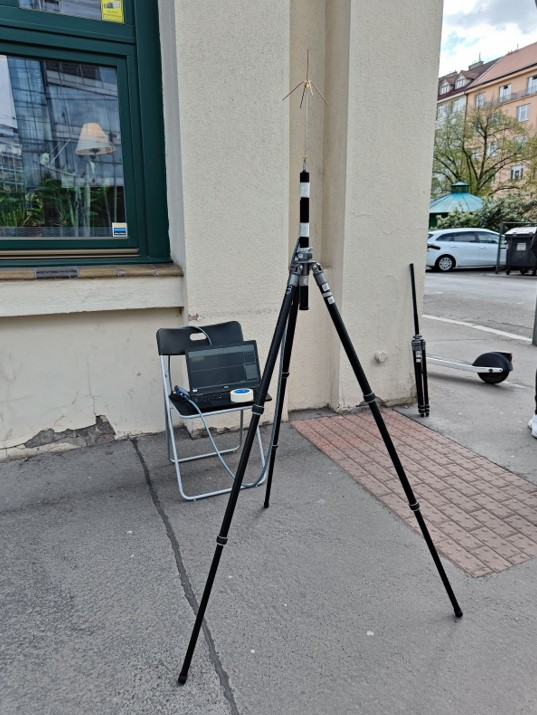
\includegraphics[,scale=0.35]{img/antenna_1.jpg}
    \caption{Vysílací stanoviště na rohu ulic Jugoslávských partyzánů a Roosveltova}
    \label{fig:my_label}
\end{figure}

\begin{figure}[h!]
    \centering
    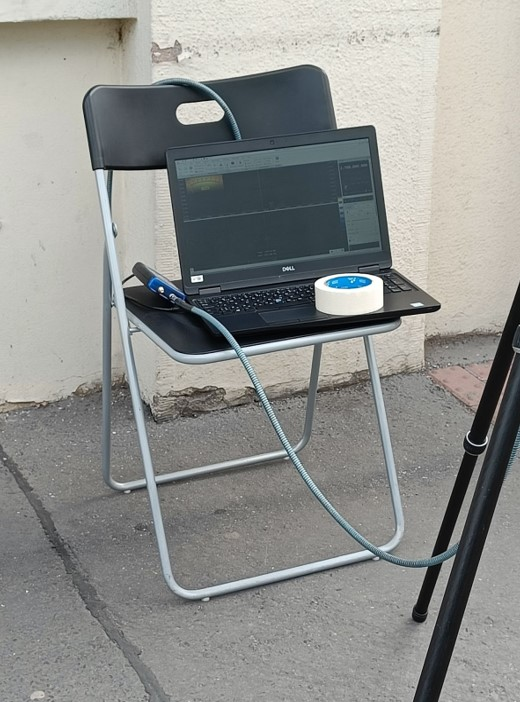
\includegraphics[,scale=0.35]{img/notebook_mereni1.jpg}
    \caption{Detail na umístění notebooku, včetně zapojení SDR}
    \label{fig:my_label}
\end{figure}

\clearpage

\begin{figure}[h!]
    \centering
    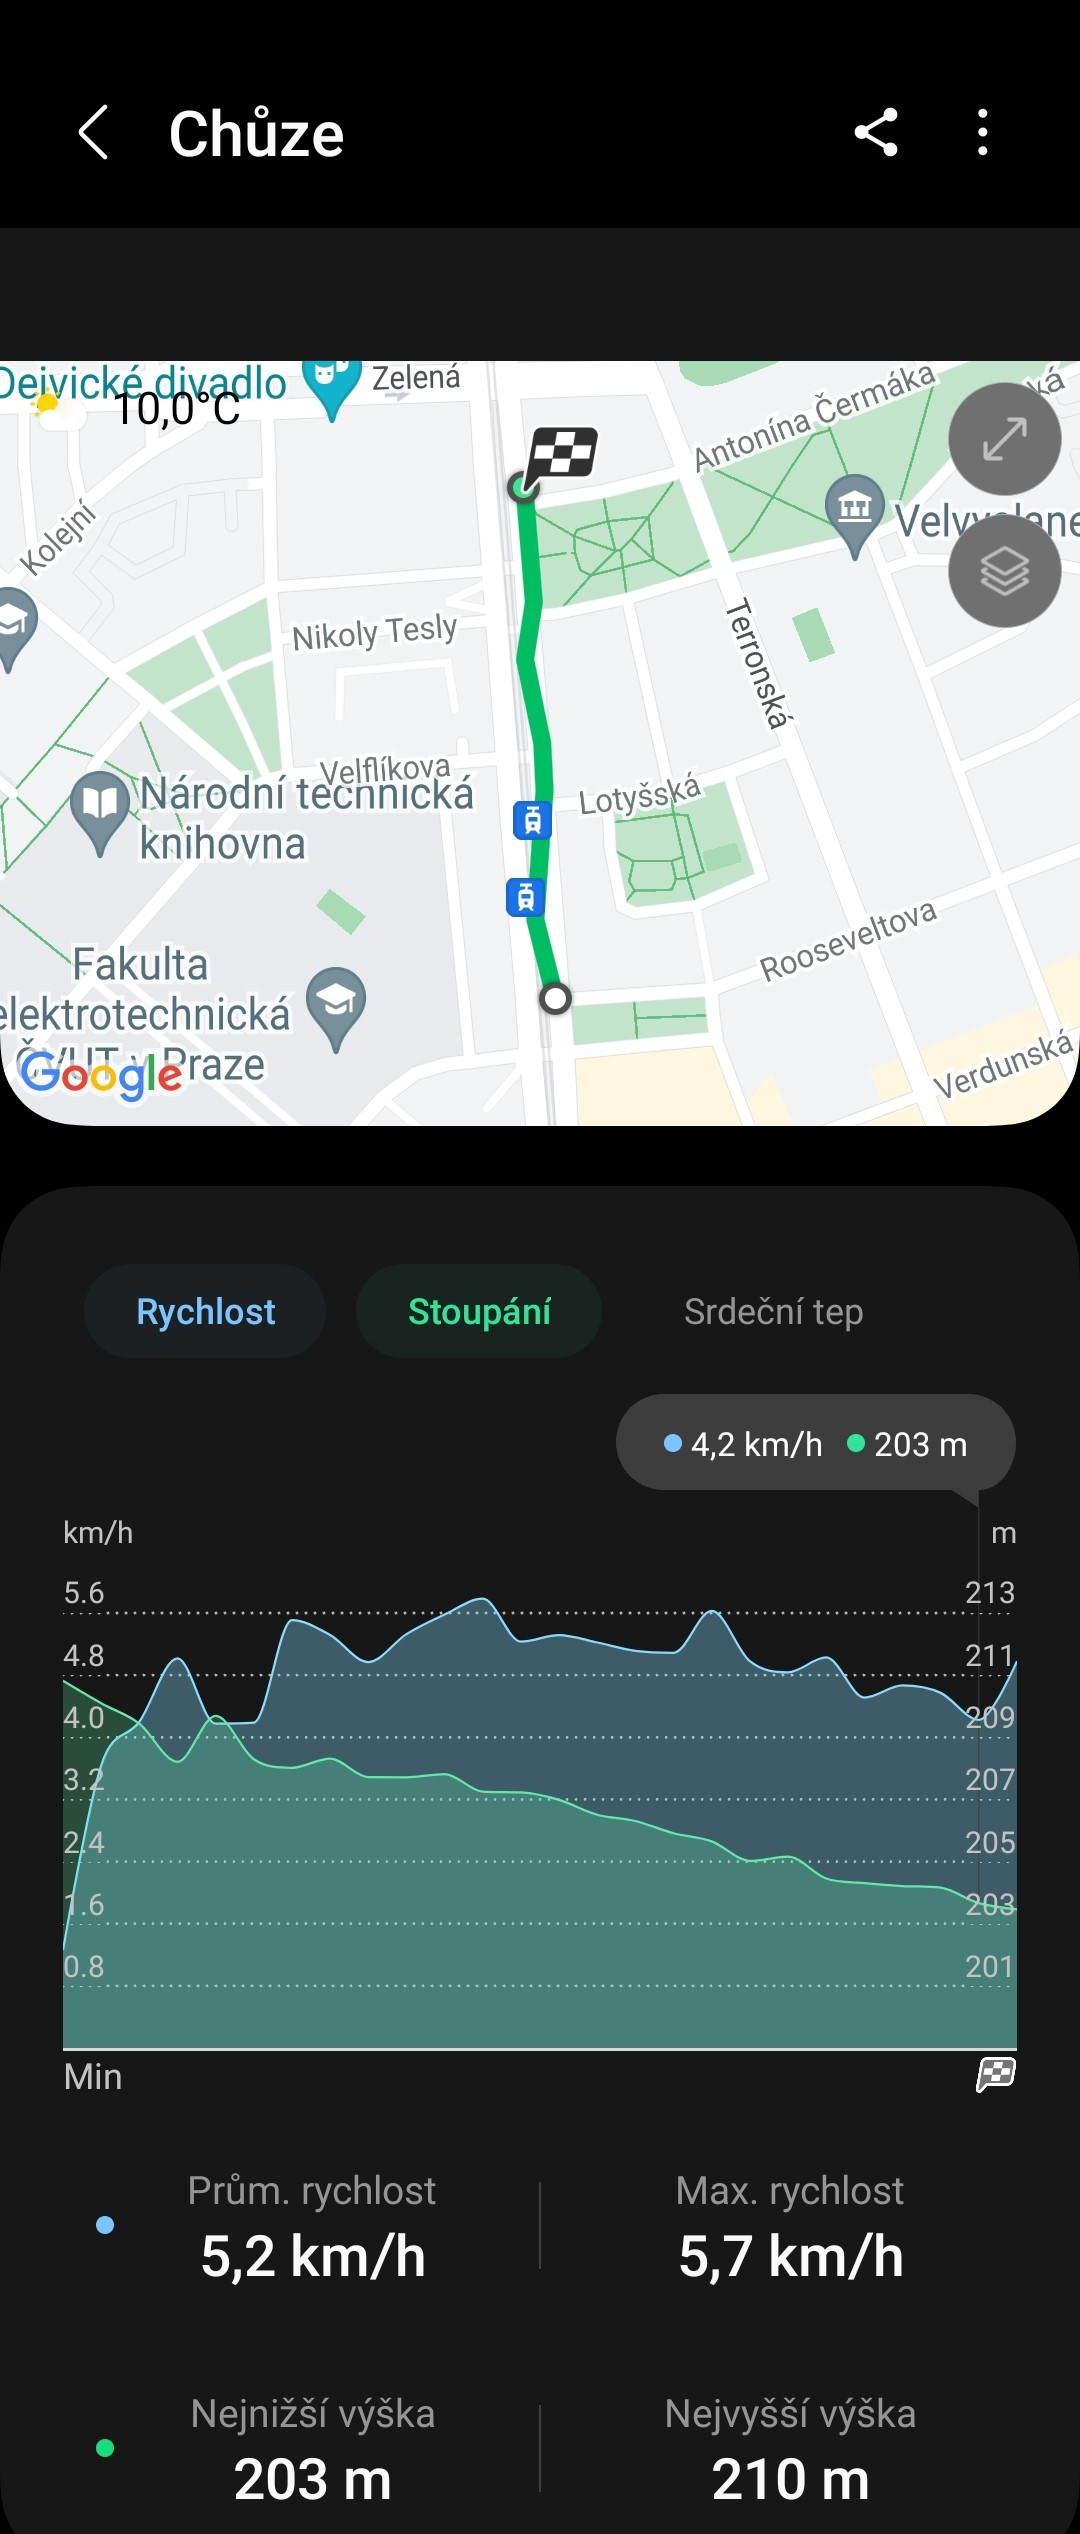
\includegraphics[,scale=0.16]{img/mereni1_cesta_tam.jpg}
    \caption{Data o vzdálenosti z GPS v mobilní aplikaci včetně rychlosti a převýšní}
    \label{fig:my_label}
\end{figure}

\begin{figure}[h!]
    \centering
    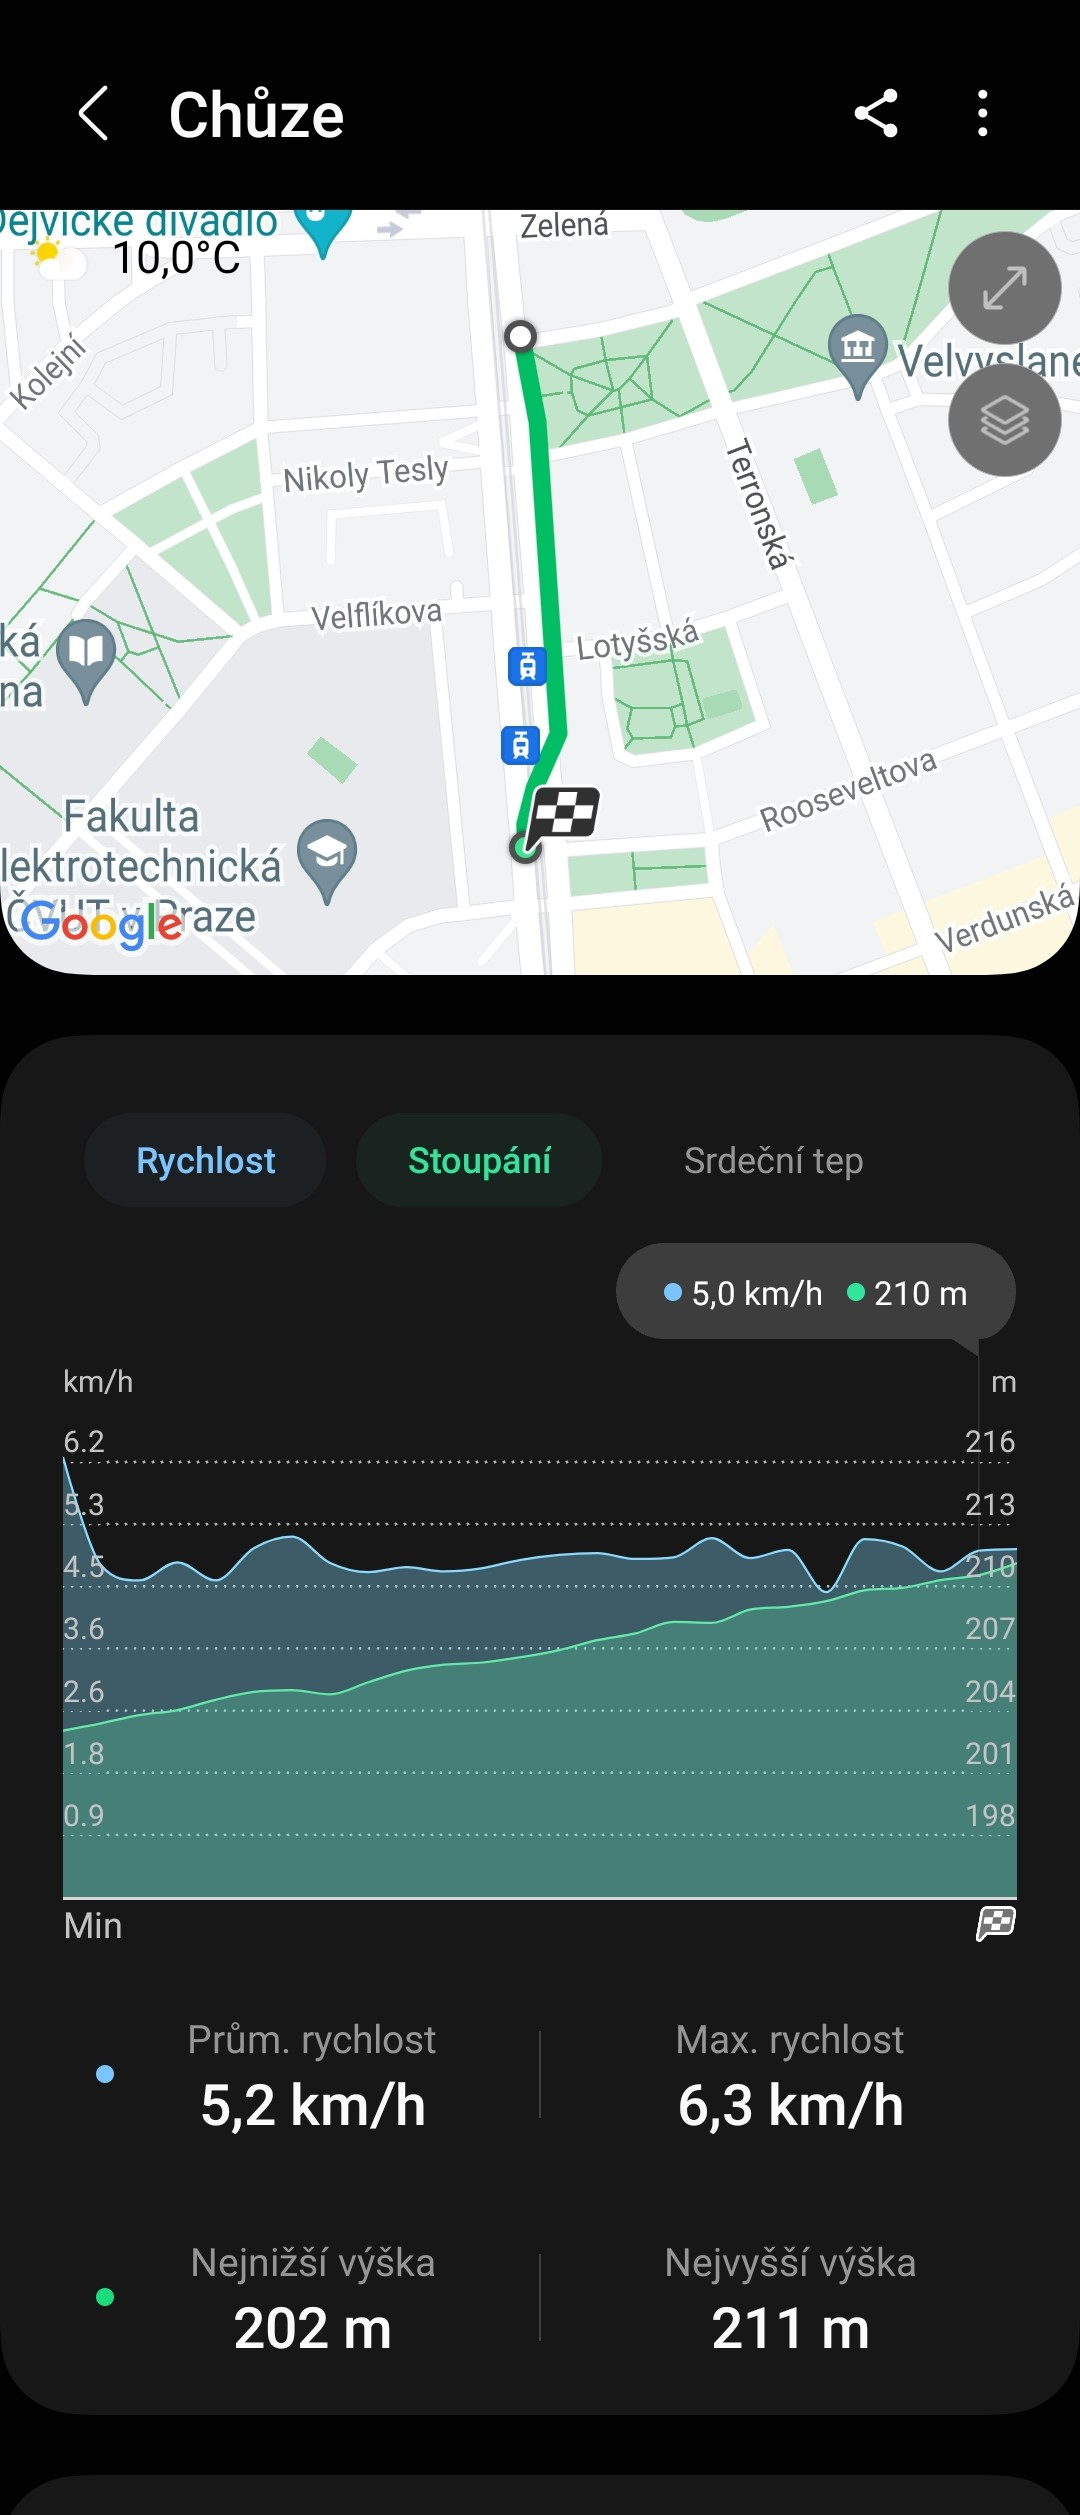
\includegraphics[,scale=0.16]{img/mereni1_Cesta_zpet.jpg}
    \caption{Data o vzdálenosti z GPS v mobilní aplikaci včetně rychlosti a převýšní pro cestu k vysílací anténě}
    \label{fig:my_label}
\end{figure}

\begin{figure}[h!]
    \centering
    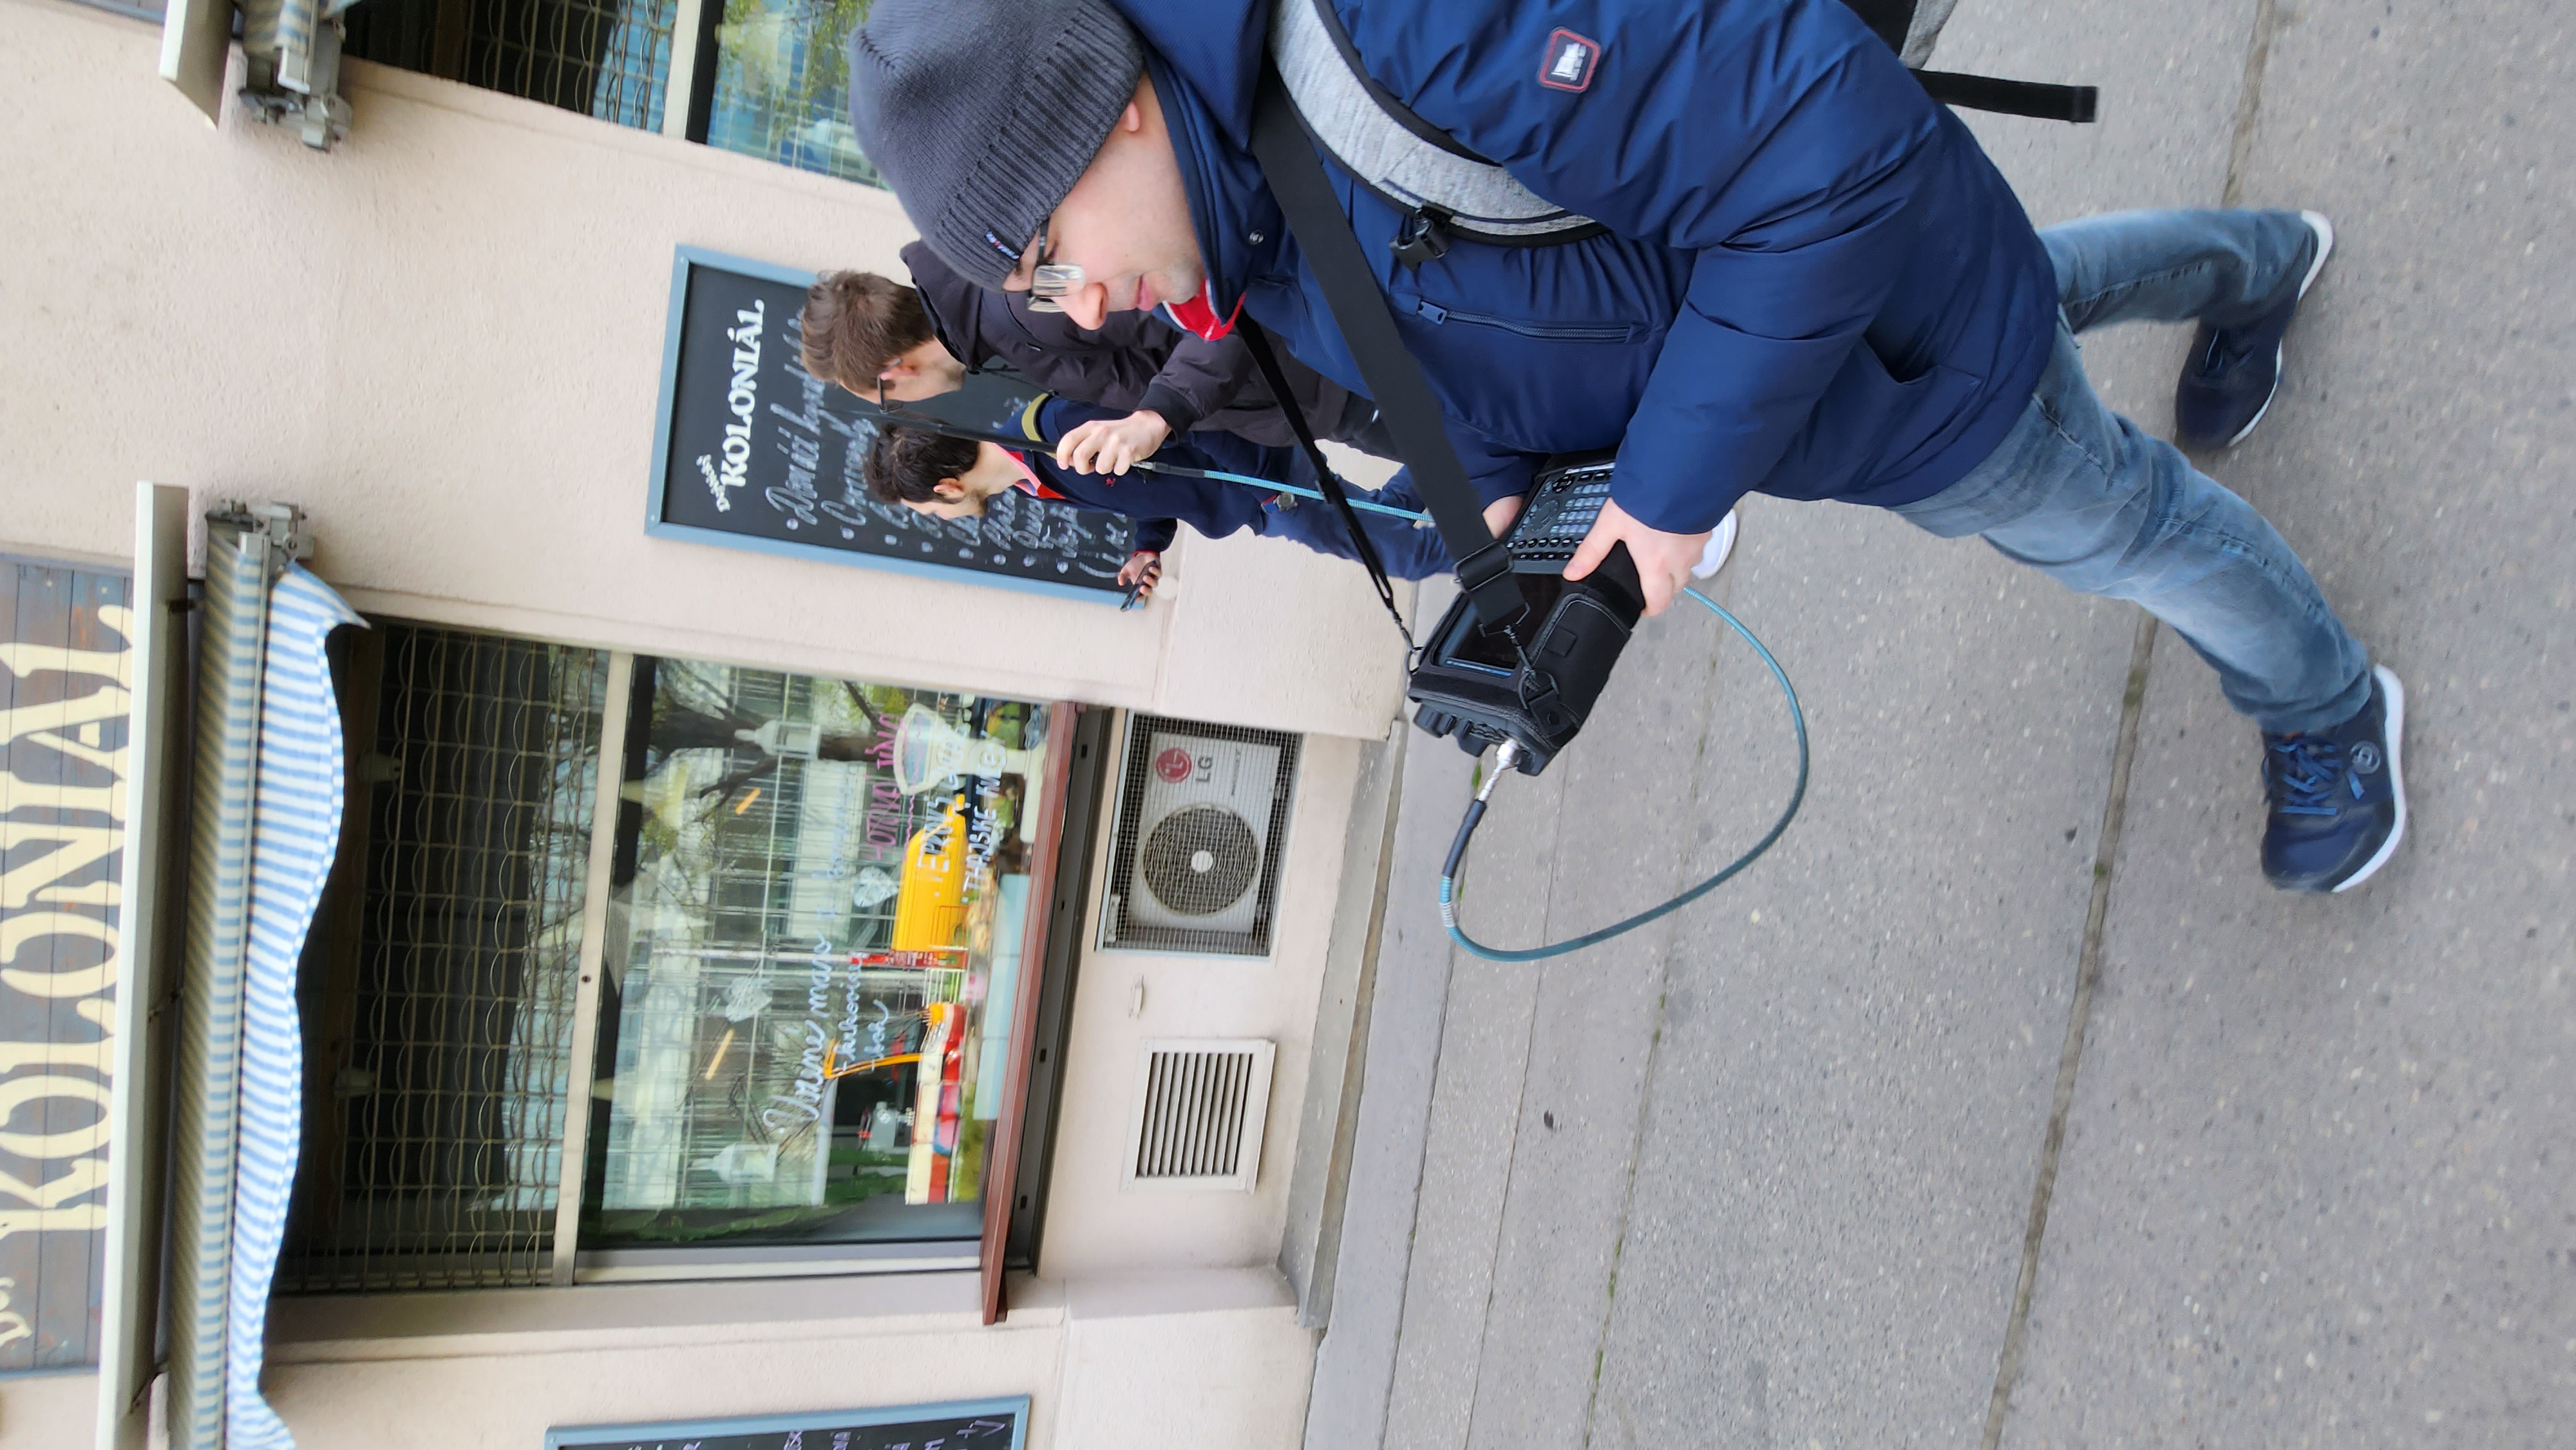
\includegraphics[angle=270,scale=0.07]{img/foto_mereni_jugoslavskych_partyzanu.jpg}
    \caption{Foto z průběhu měření v ulici Jugoslávských partyzánů}
    \label{fig:my_label}
\end{figure}

\subsection{Grafy s výsledky prvního měření}

Pro přehlednost celé práce jsou zde uvedeny grafy pouze pro měření v jednom směru. Výsledné hodnoty modelu jsou pak zprůměrováním obou měření v dané lokalitě. 

\begin{figure}[h!]
    \centering
    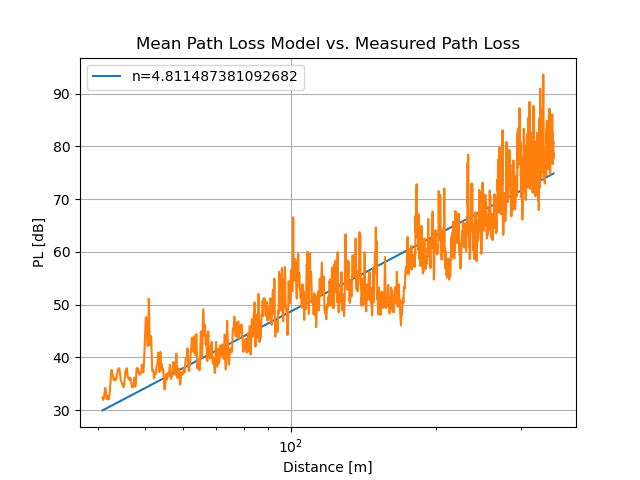
\includegraphics[,scale=0.8]{img/Mean_Path_LossVMeasured_partyzanu_dolu.png}
    \caption{Naměřená data a průběh emperického modelu}
    \label{fig:my_label}
\end{figure}

\begin{figure}[h!]
    \centering
    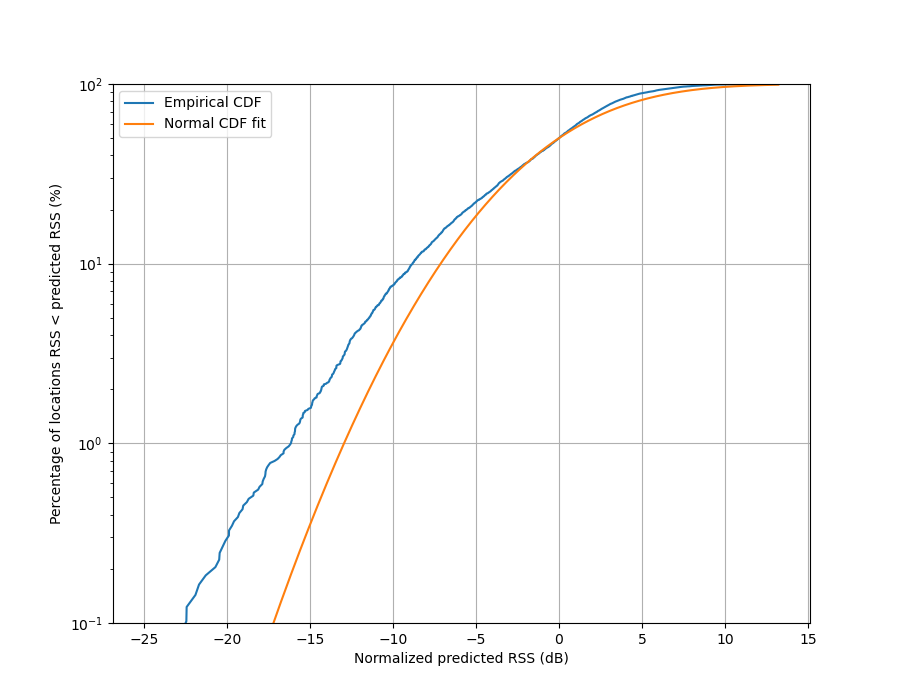
\includegraphics[,scale=0.52]{img/CDF_partyzanu.png}
    \caption{Graf zobrazující emperickou CDF a odhadnutou CDF}
    \label{fig:my_label}
\end{figure}

\begin{figure}[h!]
    \centering
    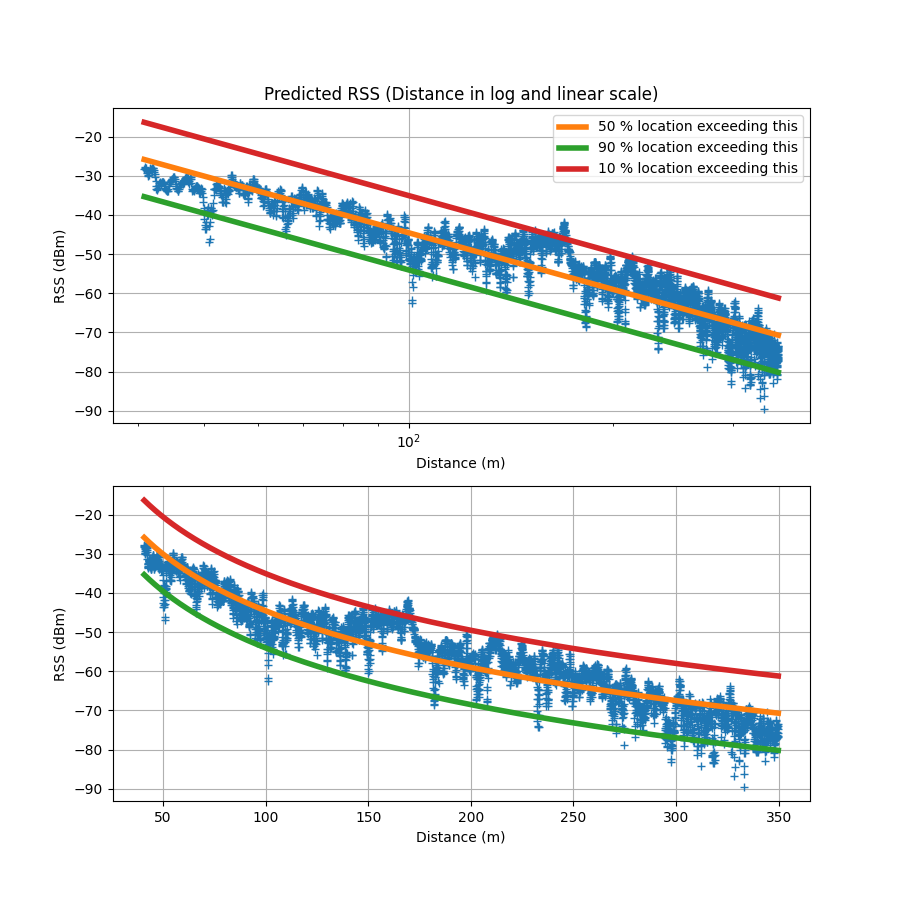
\includegraphics[,scale=0.52]{img/Prediction2partyzanu_dolu.png}
    \caption{Naměřená data společně s predikovaným průběhem modelu}
    \label{fig:my_label}
\end{figure}

\begin{figure}[h!]
    \centering
    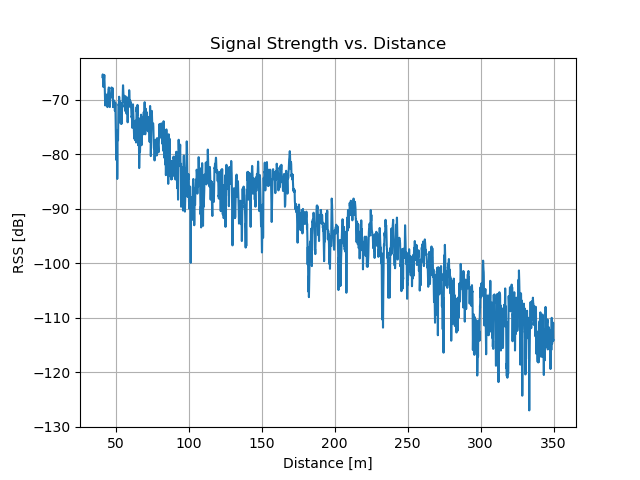
\includegraphics[,scale=0.7]{img/Signal_StrengthVDistance_partyzanu_dolu.png}
    \caption{Naměřené hodnoty síly signálu v závislosti na vzdálenosti}
    \label{fig:my_label}
\end{figure}

\begin{figure}[h!]
    \centering
    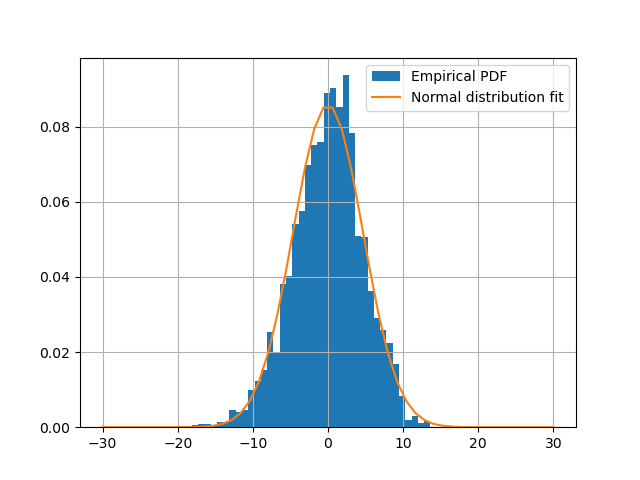
\includegraphics[,scale=0.7]{img/Statistics_partyzanu_dolu.png}
    \caption{Normálové rozdělí a jeho porovnání s rozdělením naměřených dat}
    \label{fig:my_label}
\end{figure}

\section{Měření 2. - ulice Teronská}
Druhé měření bylo také provedeno uvnitř husté zástavby, tentokrát v ulici Terronská. Měření bylo usutečněno od rohu ulice Rooseveltova na roh ulice Antonína Čermáka, kde celková trasa má 370 metrů. Výšky antén byly umístěny ve stejné výšce jako v prvním měření, tedy 170 cm nad zemí. Metodika měření byla stejná jako v 1. měření. Tato trasa se jeví jako lepší z důvodu menší rušnosti. Prakticky po celou dobu měření byla přímá viditelnost mezi jednotlivými anténami. V prvním měření z důvodu rušnější ulice se občas stalo, že nebyla přímá viditelnost z důvodu pohybu chodců, což bohužel v daný okamžik nešlo ovlivnit. Měření v této lokaci bylo provedeno dvakrát, jednou při pohybu od antény, podruhé při pohybu k anténě. Zjištěné hodnoty parametru $n$ odpovídají očekávaným hodnotám pro prostředí s hustou zástavbou.

\begin{table}[h!]
\centering
\begin{tabular}{|c|c|c|c|}
  \hline
   & Měření při pohybu od antény & Měření při pohybu k anténě & Průměr \\
  \hline
  $L_1$ & - dB & - dB & - dB\\
  \hline
  n & 4,08 & 3,53 & 3,81 \\
  \hline
  $\sigma$ & - dB & - dB & - dB \\
  \hline
\end{tabular}
\caption{Přehled parametrů pro měření v ulici Terronská}
\end{table}

Vyjdeme-li z rovnice 1.3, tak zjistíme, že pro náš případ s uvedenými výškami antén a frenkvencí vychází, že vzdálenost Fresnelova zlomu je opět 38.5 metru., protože jsme vysílali na stále stejné frekvenci a ani výška antén se zde neměnila. 
\subsection{Fotografie a záznamy hodnot z měření}

\begin{figure}[h!]
    \centering
    \includegraphics[angle=270,scale=0.06]{img/antena_terronska.jpg}
    \caption{Vysílací stanoviště v ulici Terronská s pohledem ve směru měření}
    \label{fig:my_label}
\end{figure}

\begin{figure}[h!]
    \centering
    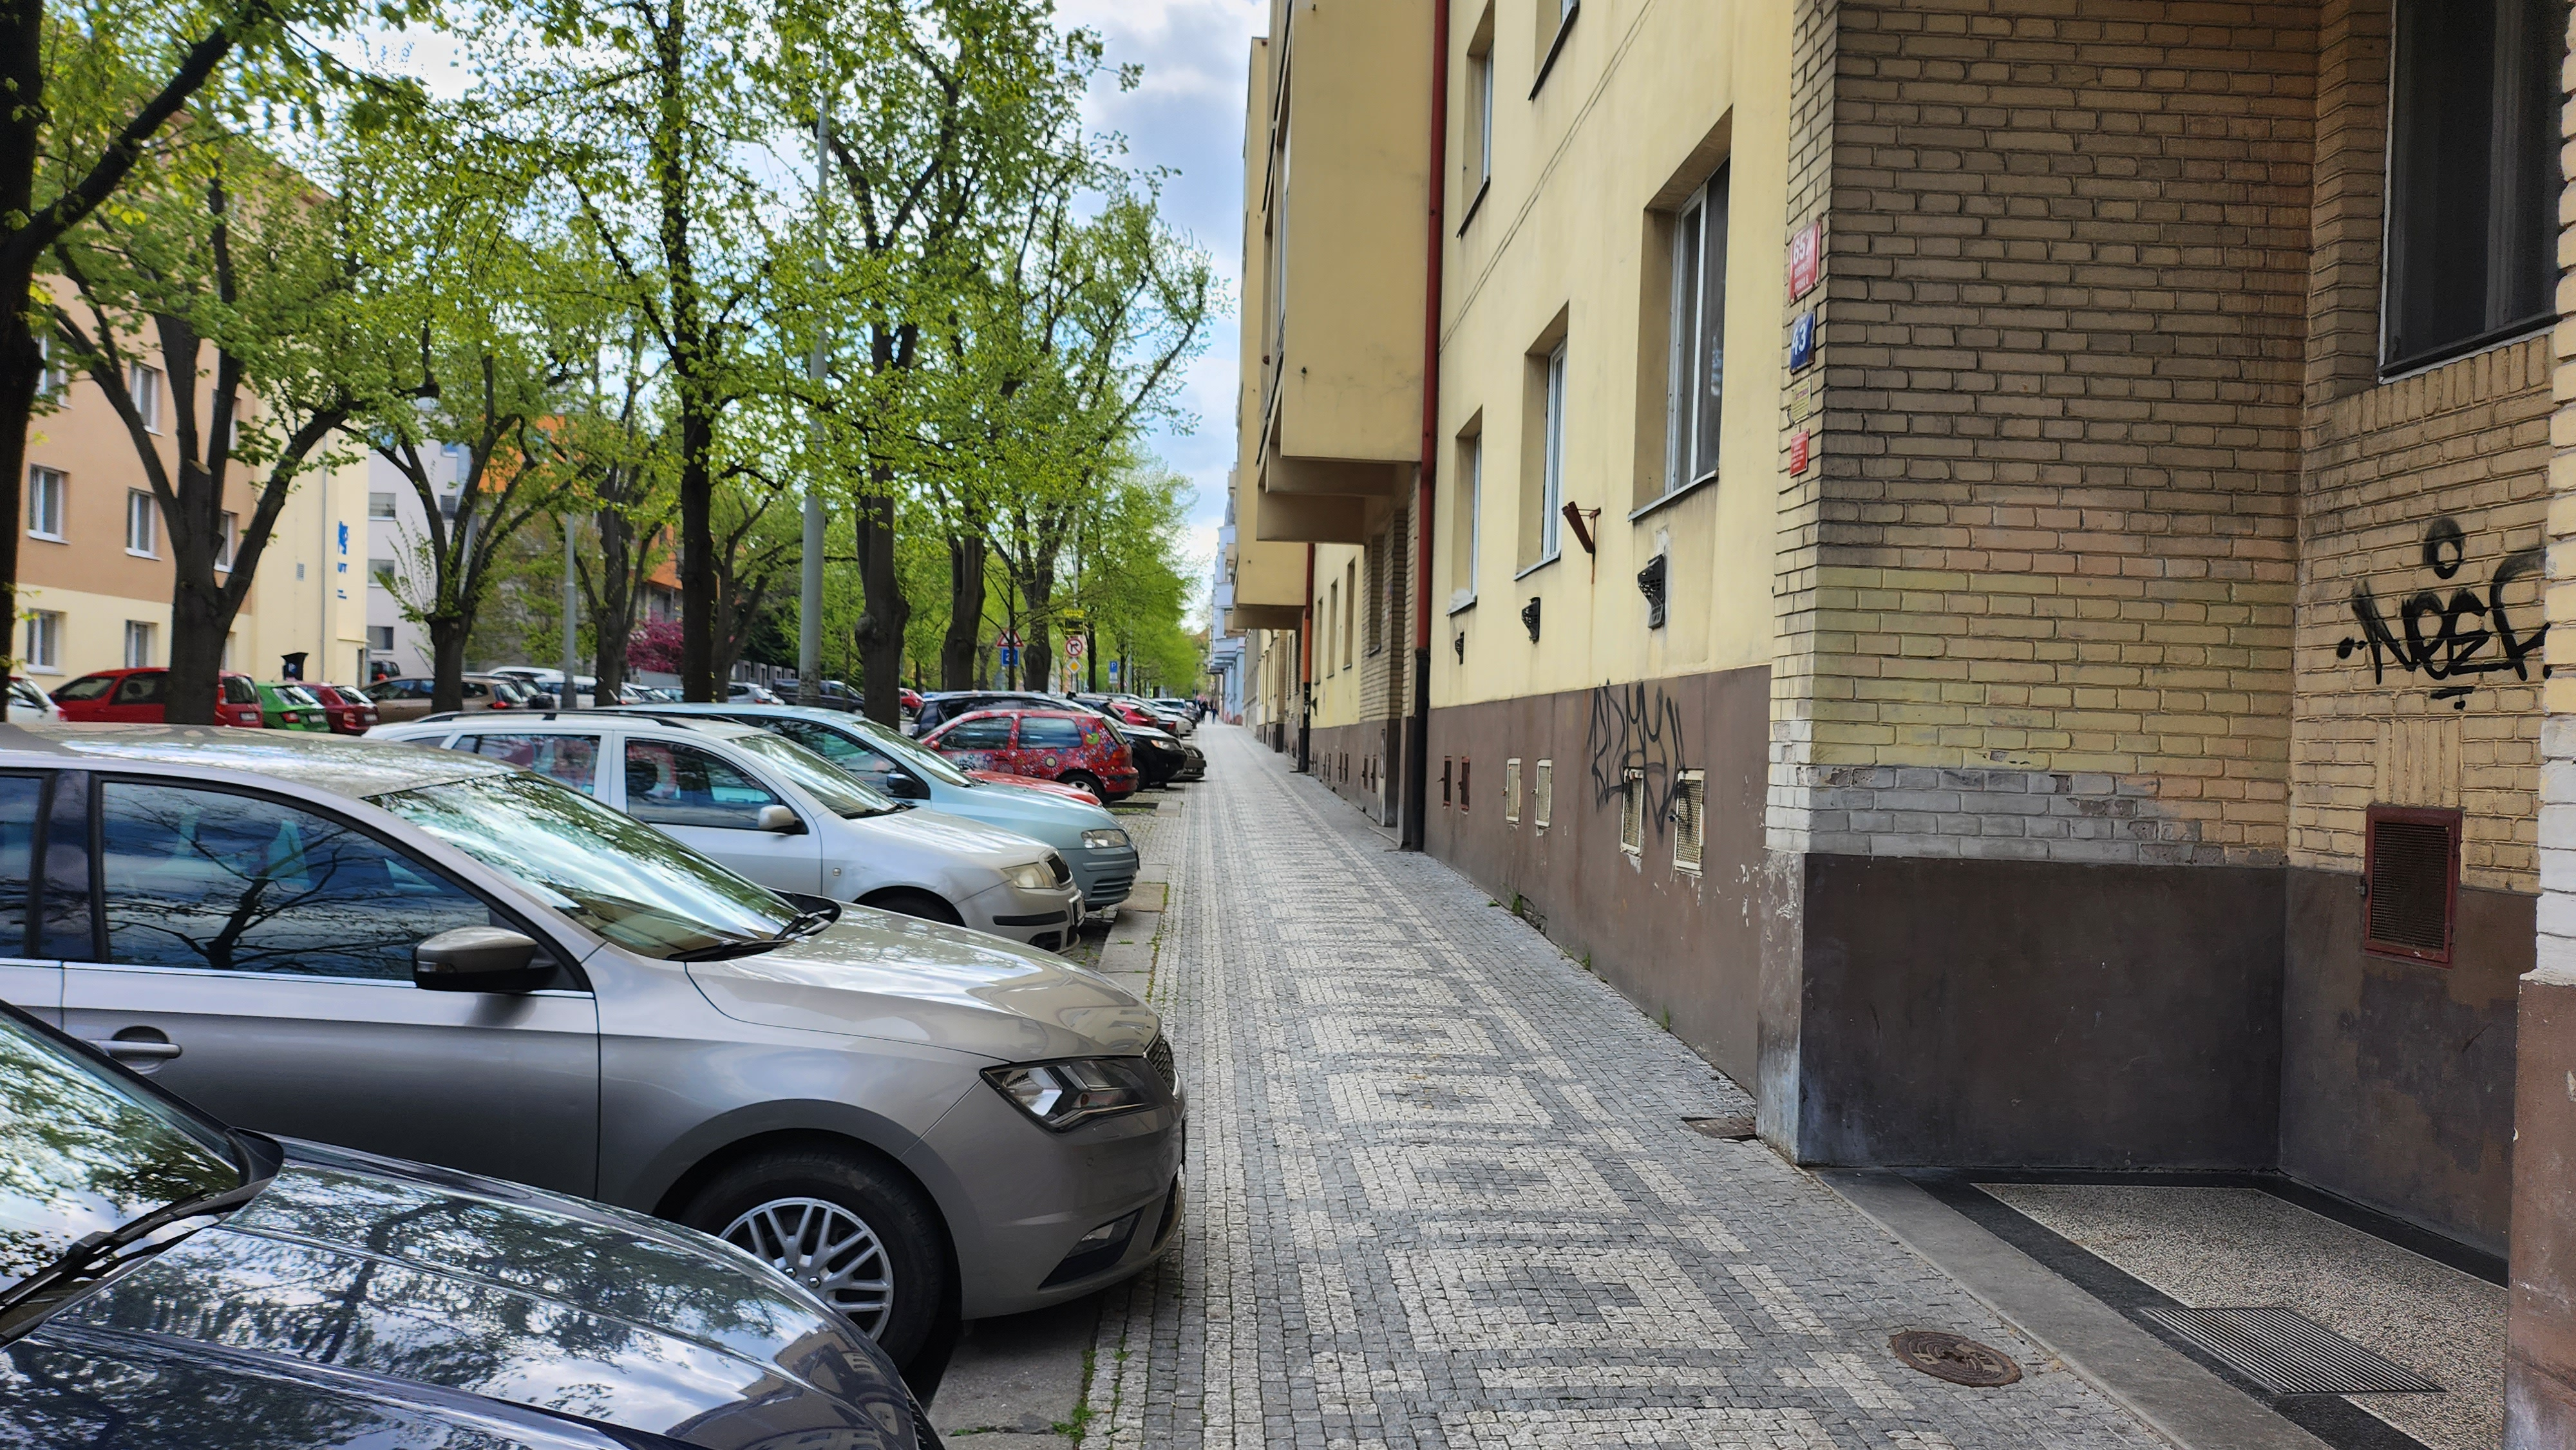
\includegraphics[,scale=0.06]{img/pohled_terronska.jpg}
    \caption{Ulice Terronská směrem k vysílací anténě}
    \label{fig:my_label}
\end{figure}

\clearpage

\begin{figure}[h!]
    \centering
    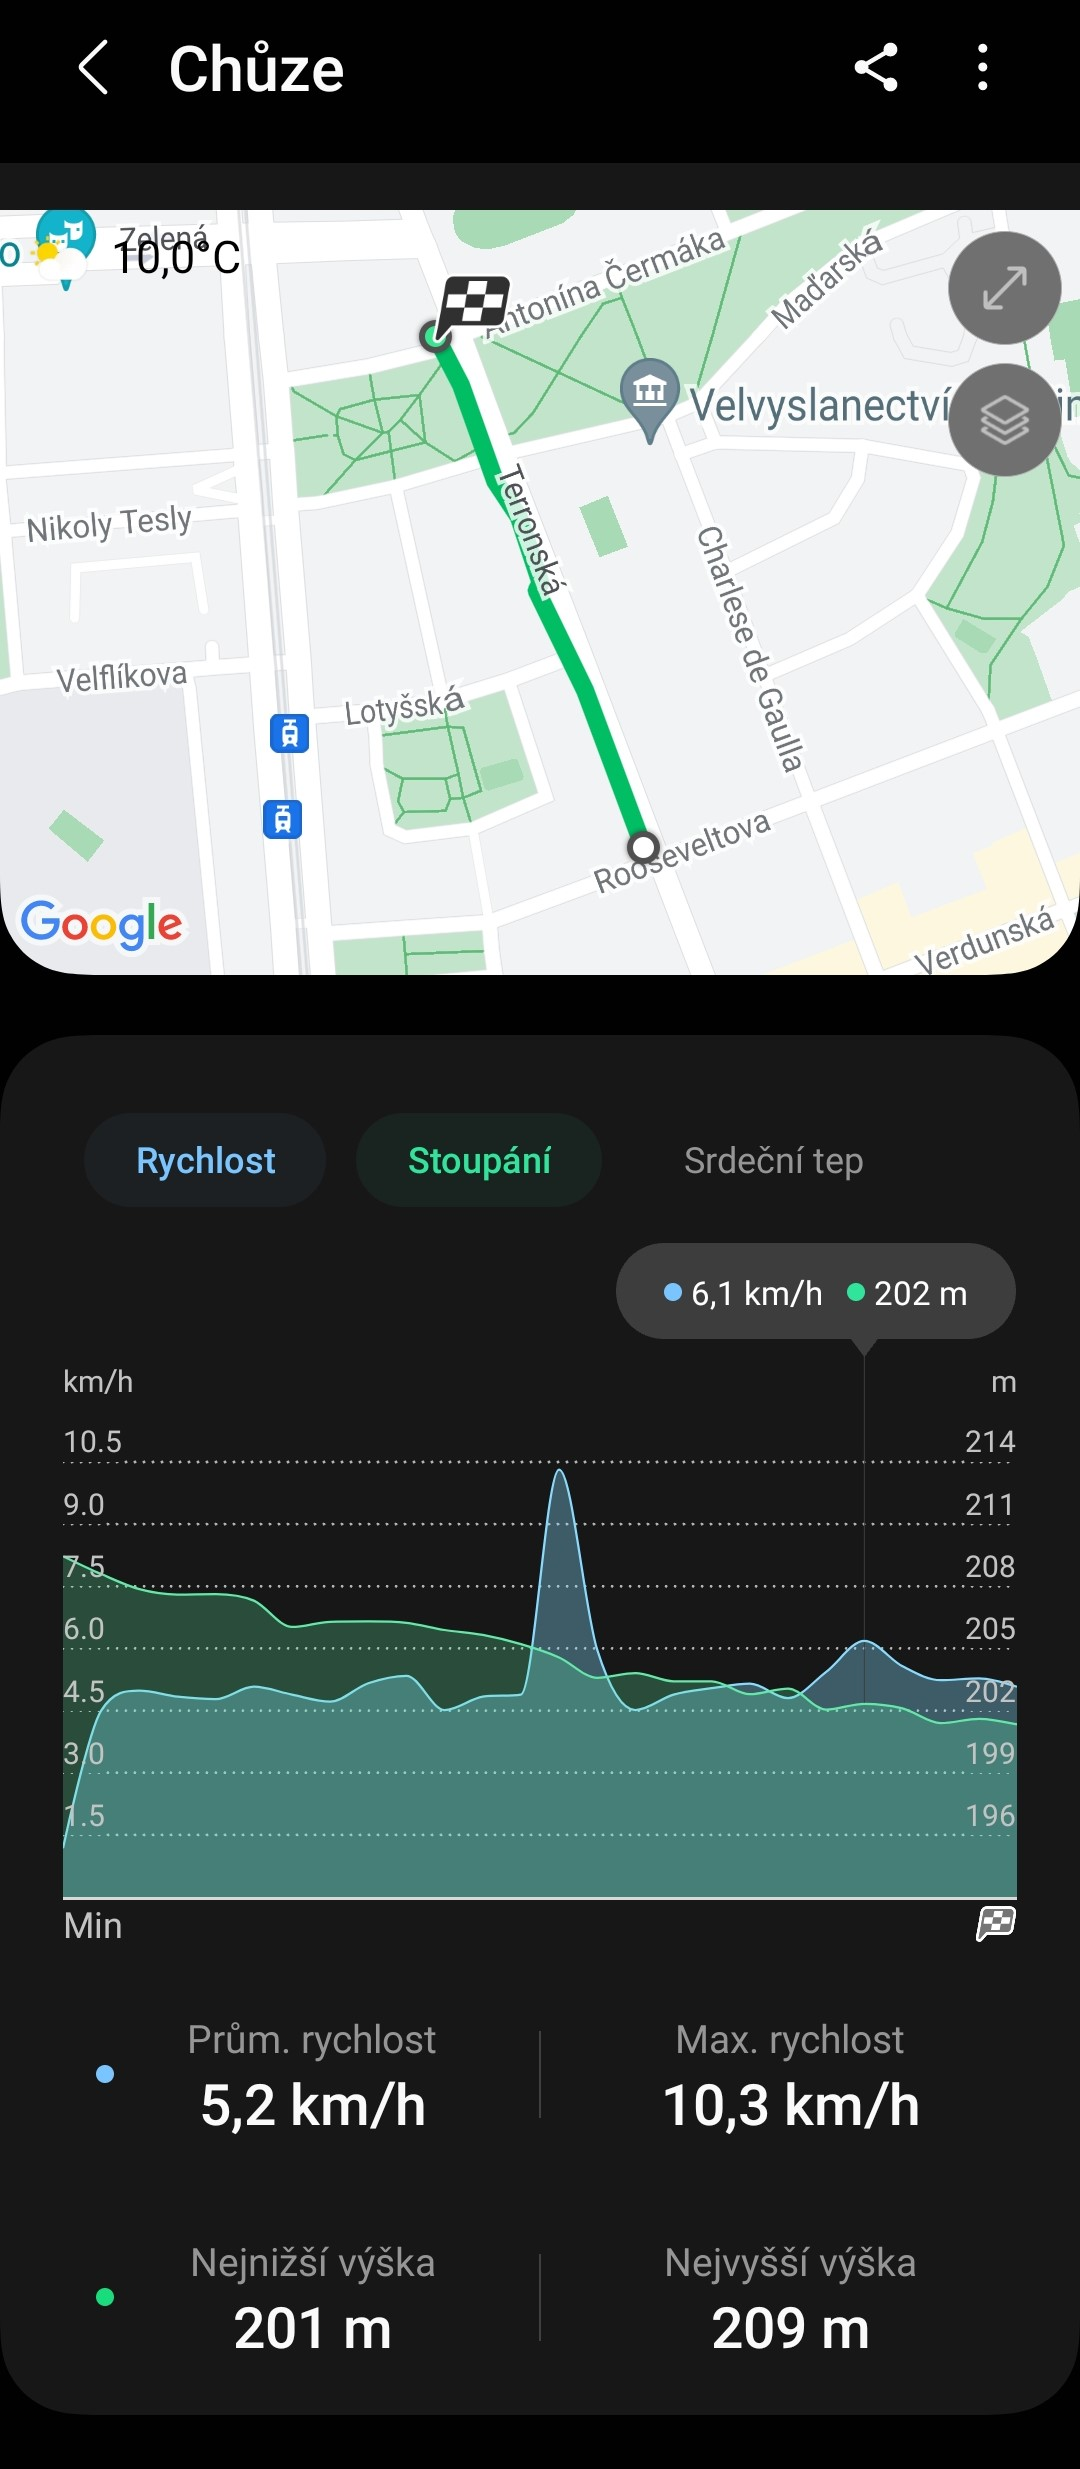
\includegraphics[,scale=0.16]{img/terronska_cestaTam.jpg}
    \caption{Data o vzdálenosti z GPS v mobilní aplikaci včetně rychlosti a převýšní}
    \label{fig:my_label}
\end{figure}

\begin{figure}[h!]
    \centering
    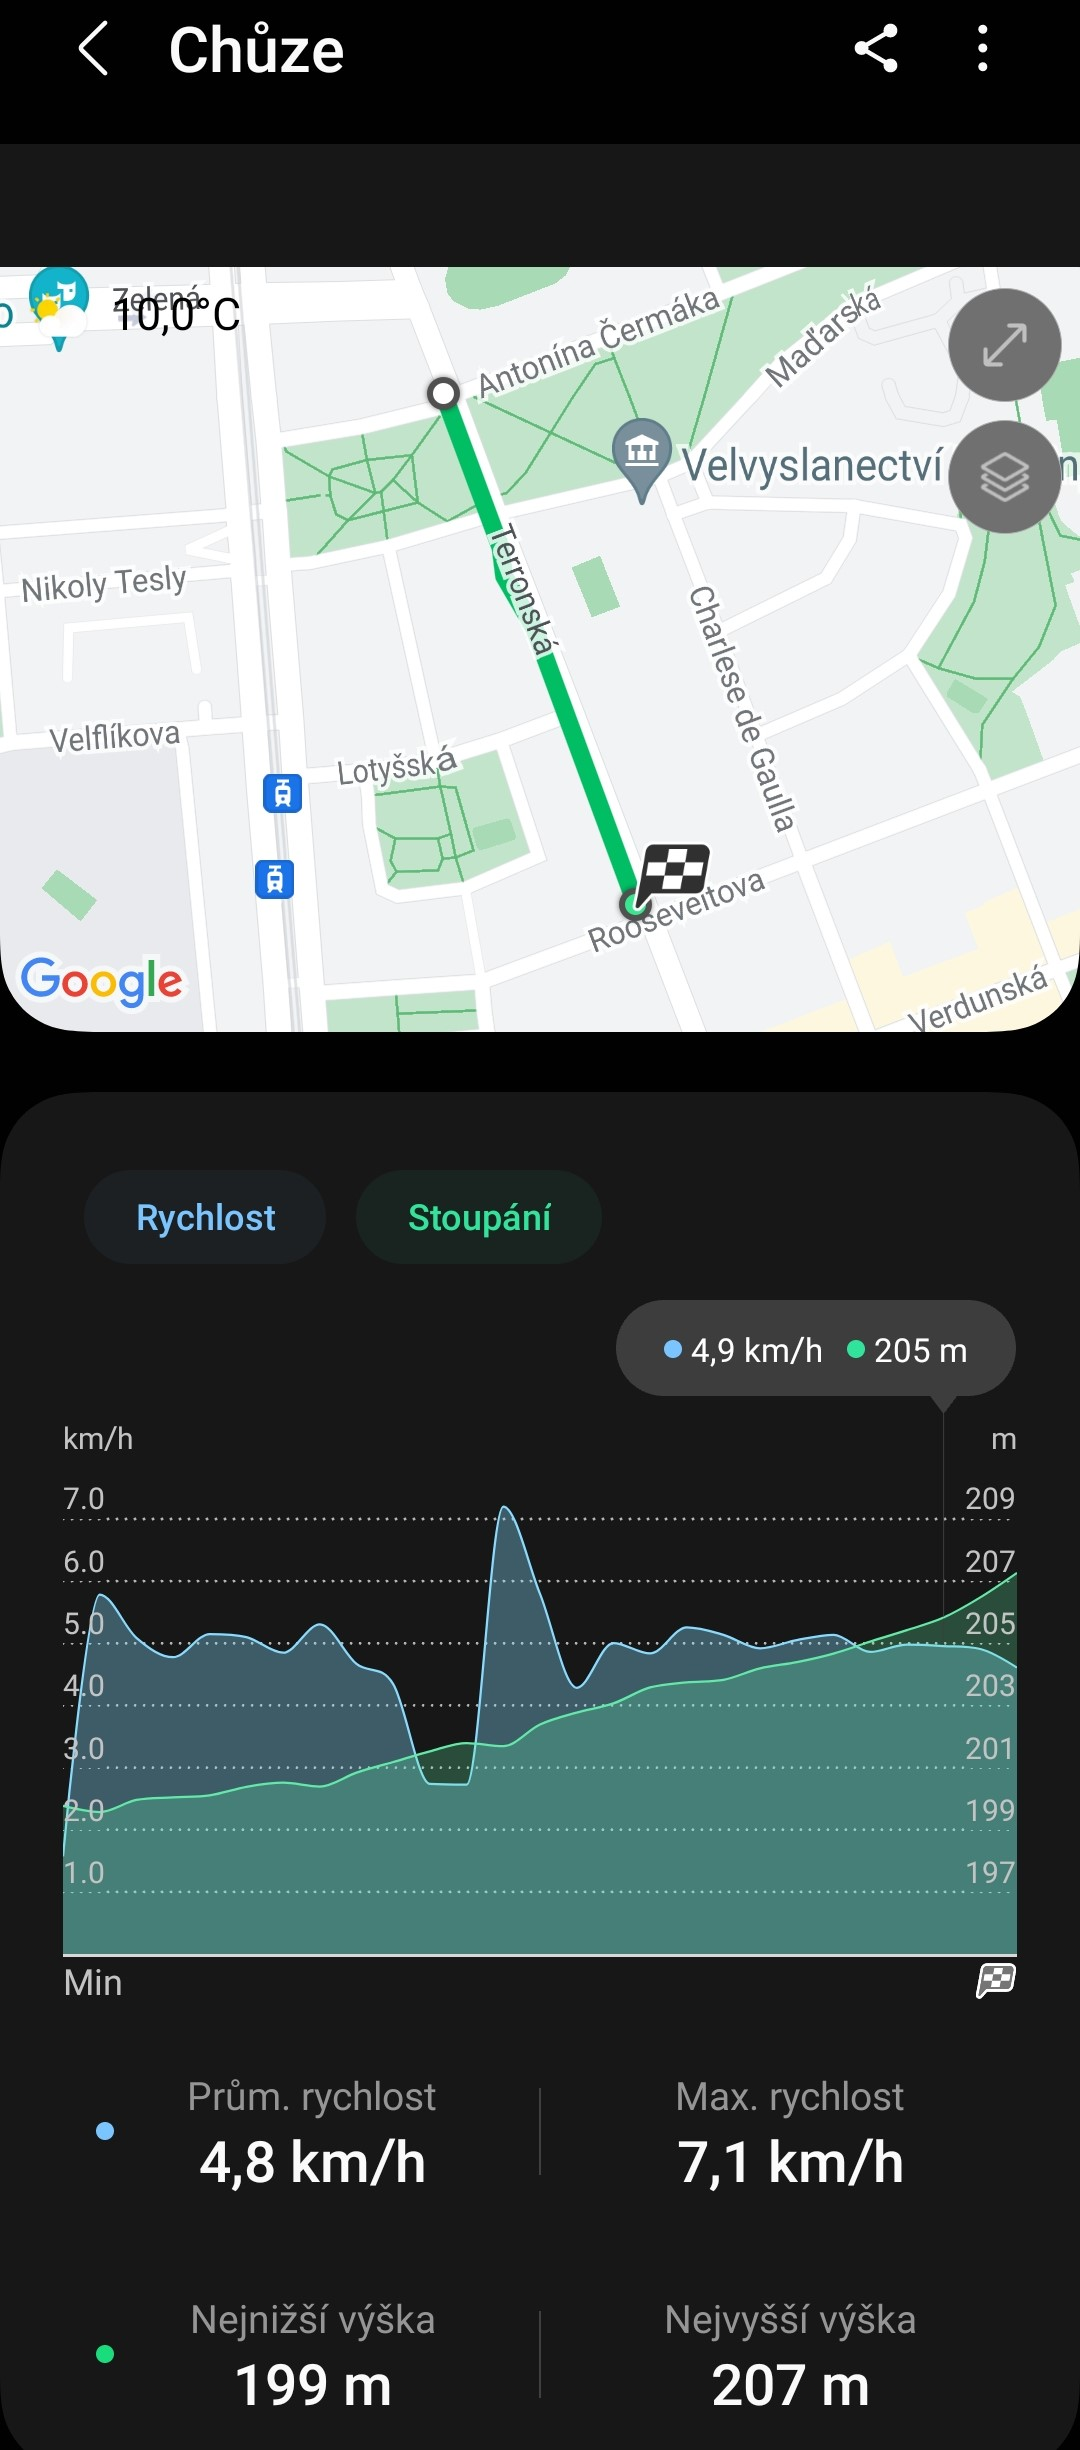
\includegraphics[,scale=0.16]{img/terronska_cesta_zpet.jpg}
    \caption{Data o vzdálenosti z GPS v mobilní aplikaci včetně rychlosti a převýšní pro cestu k vysílací anténě}
    \label{fig:my_label}
\end{figure}

\begin{figure}[h!]
    \centering
    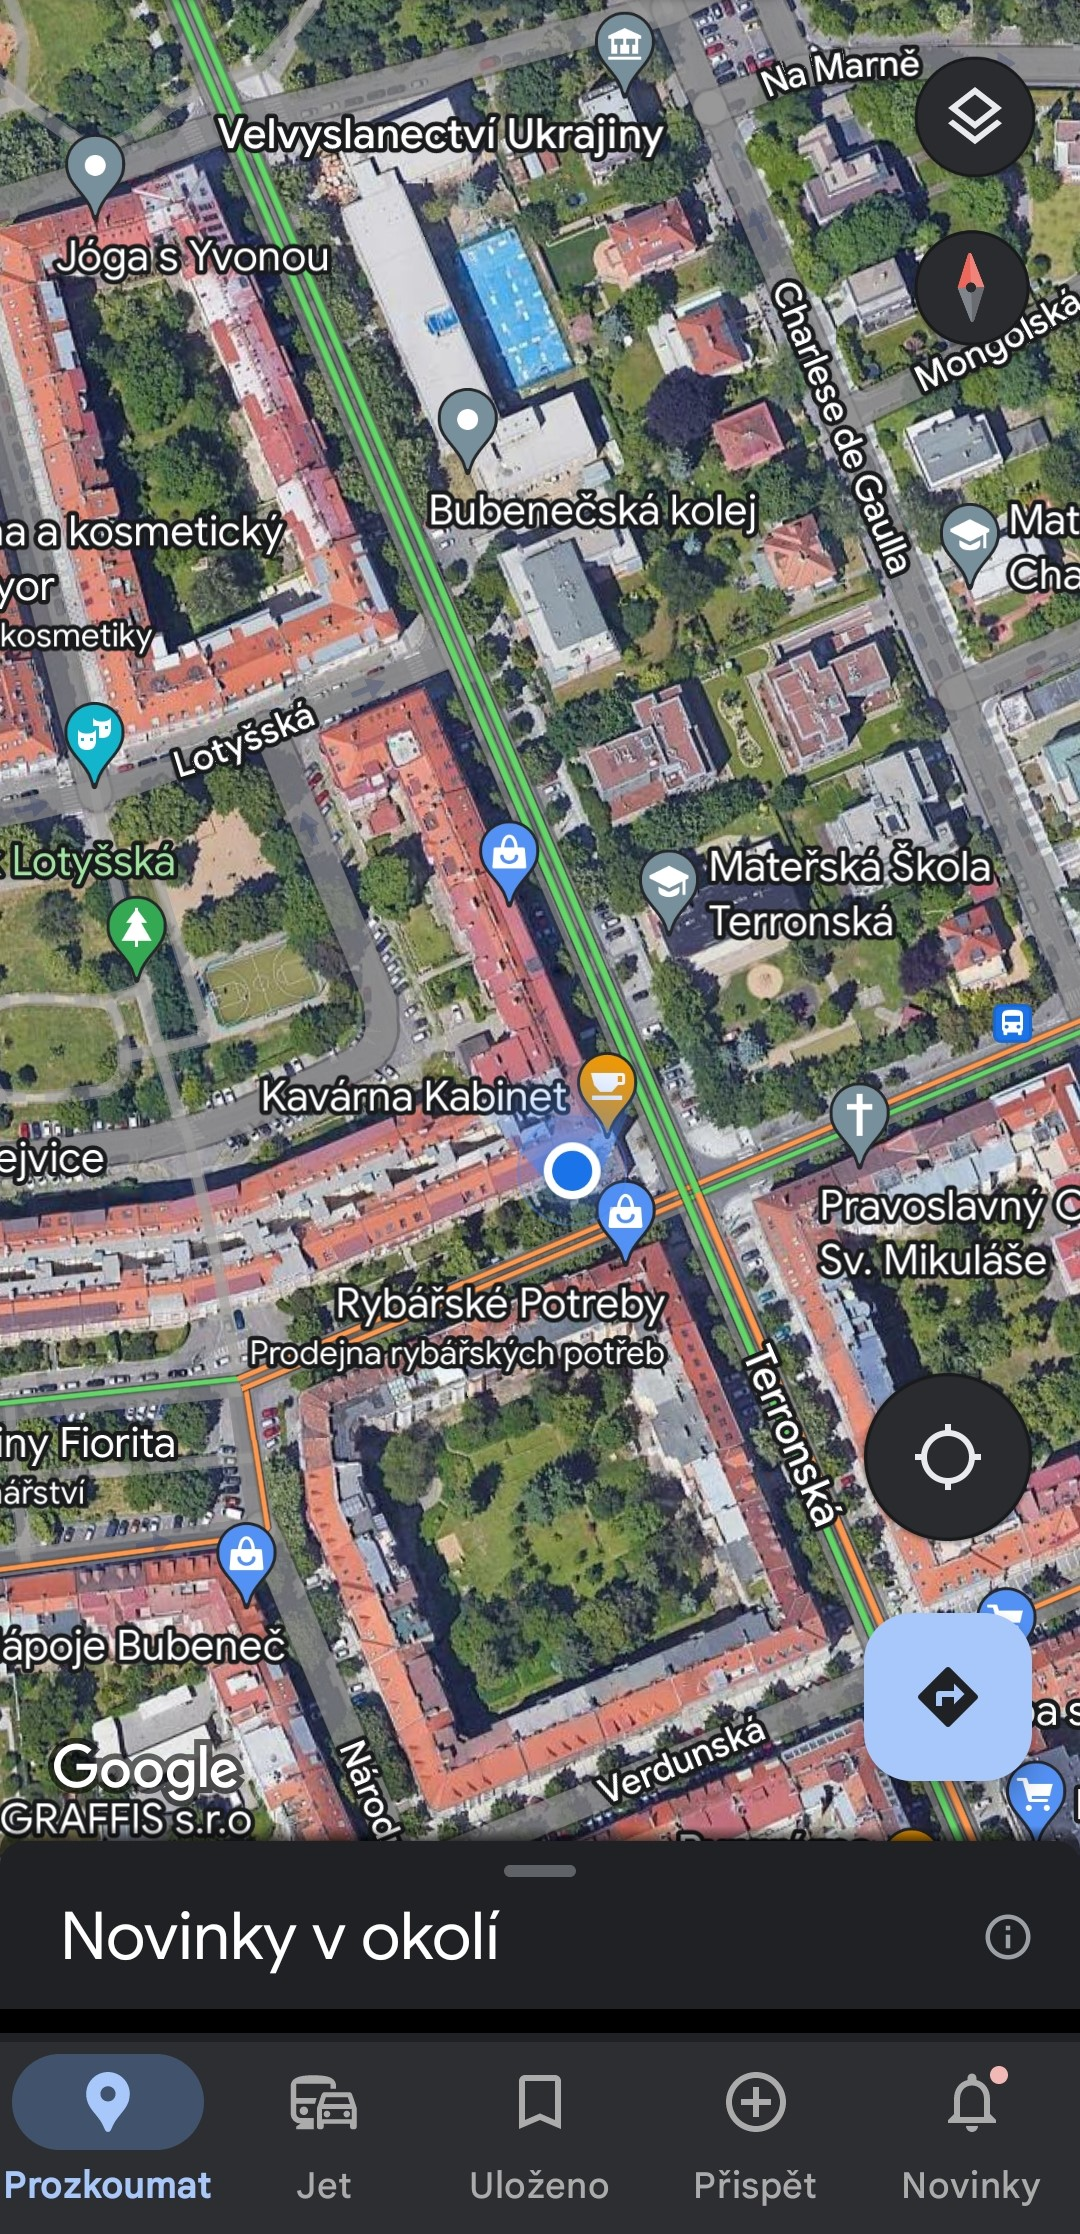
\includegraphics[,scale=0.16]{img/terronska_Satelitnisnimek.jpg}
    \caption{Satelitní snímek měřené trasy s hrubým poznačením vysílací antény}
    \label{fig:my_label}
\end{figure}

\subsection{Grafy s výsledky druhého měření}

Pro přehlednost celé práce zde opět uvádíme pouze grafy vztažené k měření při pohybu přijímací antény směrem od vysílače (jako i pro měření v ulici Jugoslávských partyzánů. Výsledné hodnoty modelu jsou pak zprůměrováním obou měření v dané lokalitě.


\begin{figure}[h!]
    \centering
    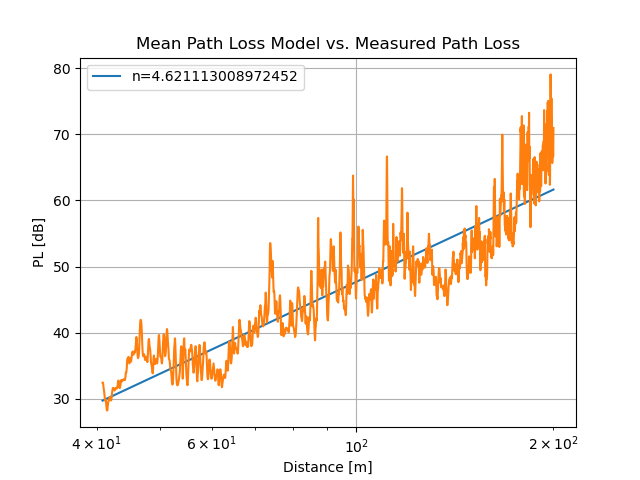
\includegraphics[,scale=0.75]{img/Mean_Path_LossVMeasured_terronska_dolu.png}
    \caption{Naměřená data a průběh emperického modelu}
    \label{fig:my_label}
\end{figure}

\begin{figure}[h!]
    \centering
    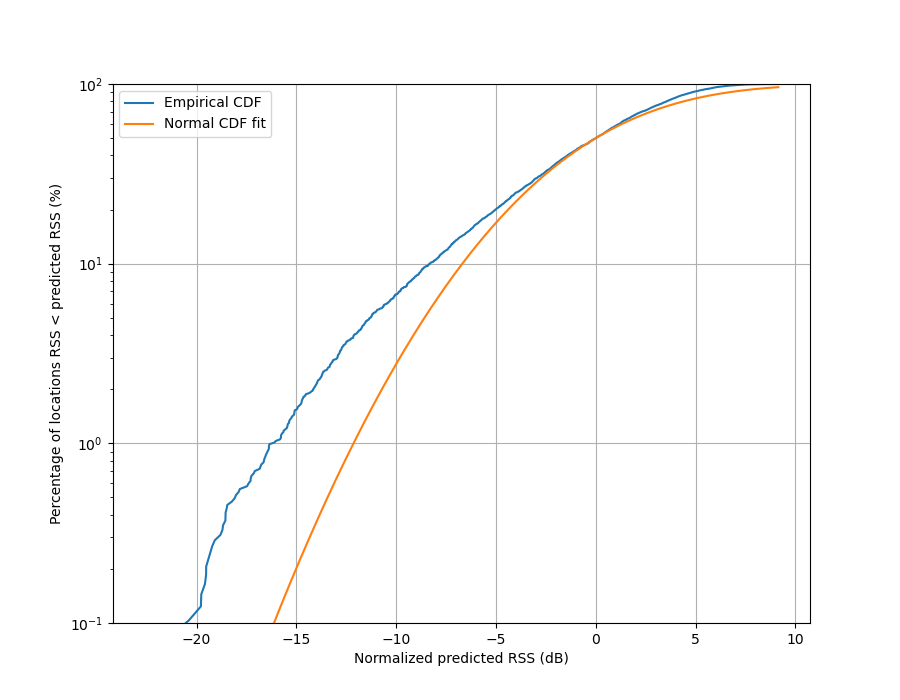
\includegraphics[,scale=0.52]{img/CDF_terronska.png}
    \caption{Graf zobrazující emperickou CDF a odhadnutou CDF}
    \label{fig:my_label}
\end{figure}

\begin{figure}[h!]
    \centering
    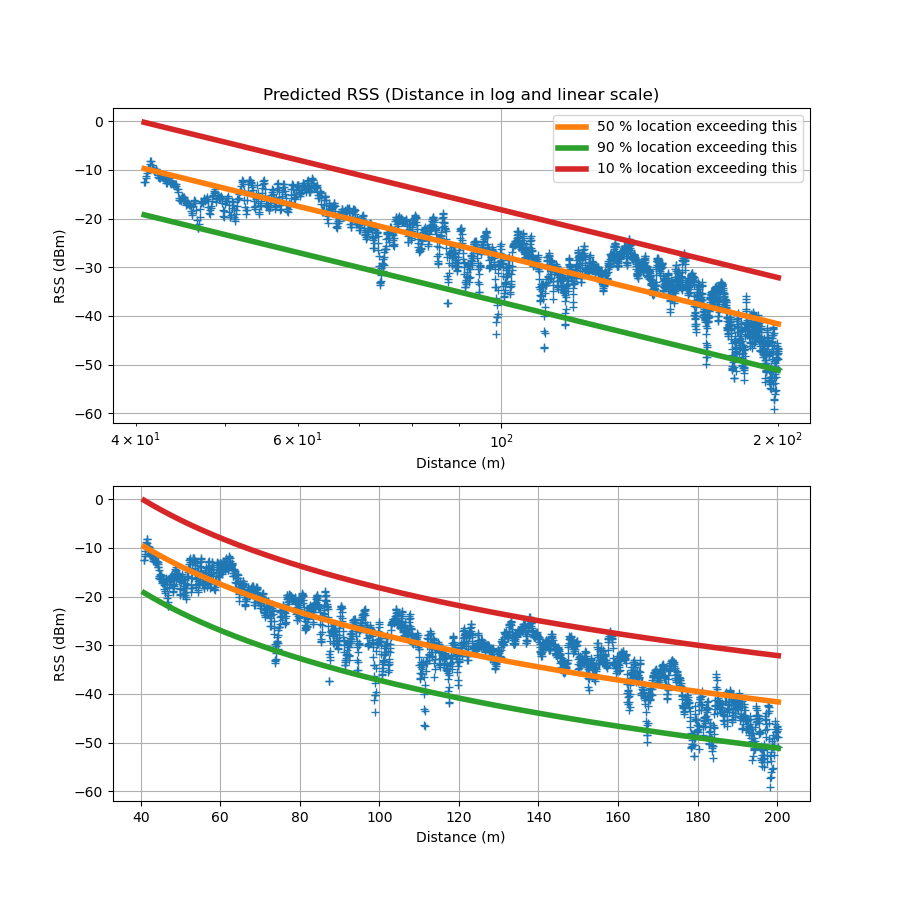
\includegraphics[,scale=0.52]{img/Prediction2terronska_dolu.png}
    \caption{Naměřená data společně s predikovaným průběhem modelu}
    \label{fig:my_label}
\end{figure}

\begin{figure}[h!]
    \centering
    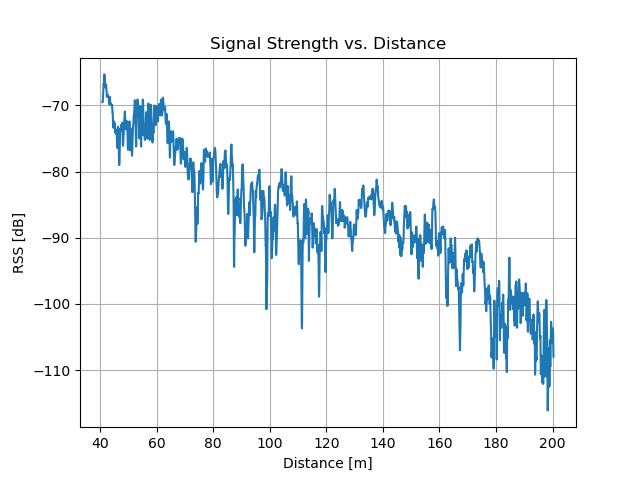
\includegraphics[,scale=0.7]{img/Signal_StrengthVDistance_terronska_dolu.png}
    \caption{Naměřené hodnoty síly signálu v závislosti na vzdálenosti}
    \label{fig:my_label}
\end{figure}

\begin{figure}[h!]
    \centering
    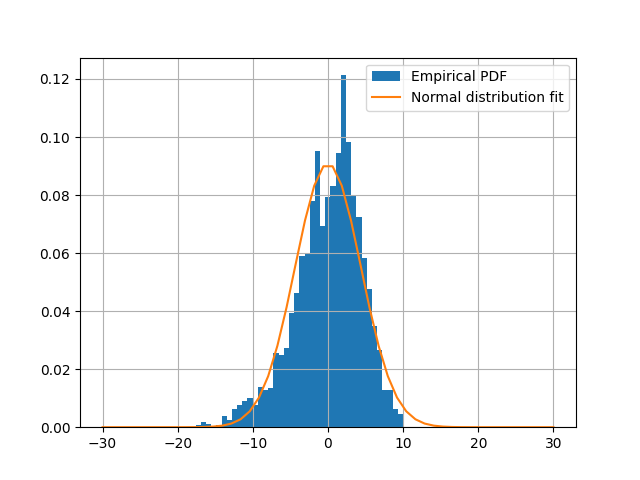
\includegraphics[,scale=0.7]{img/Statistics_terronska_dolu.png}
    \caption{Normálové rozdělí a jeho porovnání s rozdělením naměřených dat}
    \label{fig:my_label}
\end{figure}

\section{CO CHYBÍ V MĚŘENÍ-I}
\begin{enumerate}
    \item Výkonová bilance
    \item výsledný model u měření Terronská
    \item výsledný model u měření Jugoslávská
    \item Diskuse za celé toto měření I
\end{enumerate}





\chapter{Úniky způsobené vícecestným šířením}
Pro tento typ měření jsme potřebovali lokaci, kde bude velký pohyb chodců. Nejlépe takovou, aby docházelo k zastínění, ale také, aby zde ve vhodnou chvíli pohyb nebyl žádný nebo jen minimální. Nakonec jsme se rozhodli provést měření před vchodem do Technické menzy v Dejvicích. Čas měření nám velice vyhovoval, jelikož v tuto dobu - kolem 12. hodiny - je zde největší hustota lidí. Vzdálenost mezi anténami byla při měření 24 metrů a jednotlivé antény byly umístěny ve výšce 1,4 metru.

Obrazek anteny

Obrazek menzy - vchodu

\section{Měření bez zastínění}
Pro tento typ měření jsme se snažili najít vhodnou chvíli, kdy se mezi anténami nebude nikdo pohybovat. Bohužel se nám nepodařilo najít delší úsek, alespoň minutový, kdy by byly ideální podmínky. Z tohoto důvodu jsme vybrali několik úseků z více měření, které splňovali toto kritérium a tyto úseky jsme následně spojili.

Tabulka

Tabulka

Obrazek - Distribuční funkce bez zastínění - DETAILNĚJŠÍ (druhou vymazat)

Obrazek - normalikovane hodnoty v case

Obrazek - nenormalizovaný ???????????????????

\section{Případ dynamického zastínění}
Pro tento typ měření jsme záměrně volili intervaly, kdy se budou mezi anténami pohybovat v dostatečném počtu lidé. Takový interval nebylo těžké nalézt, a to ani dokonce v dostatečně dlouhém časovém intervalu, který jsme si na začátku měření stanovili.

Tabulka

Tabulka

Obrazek - Distribuční funkce bez zastínění - DETAILNĚJŠÍ (druhou vymazat) A TU JEDNU NUTO OPRAVIT!!!

Obrazek - normalikovane hodnoty v case - VYSTREDIT VUCI STREDNI HODNOTE

Obrazek - nenormalizovaný ??????????????????? - STREDNI HODNOTA!!!

\section{Případ úplného zastínění}
Při tomto scénáři jsme se snažili najít takový okamžik, kdy bylo co největší zastínění mezi anténami. Největší zastínění se nám podařilo získat, když většina osob procházela dveřmi do menzy. Navíc, my jako členové týmu jsme se pohybovali mezi anténami pro zvýšení efektu. Bohužel se nám nepodařilo zachytit dostatečně dlouhý úsek, kdy by došlo k úplnému zastínění. Z toho důvodu jsme vybrali z měření kratší úsek, který byl pro další analýzu vložen vícekrát za sebe. Tím dojde alespoň k vyhlazení křivky. Kolega, který nás měl na starost, nám sám řekl, že v tomto scénáři je úplné zastínění velice těžko proveditelné, ač jsme se snažili sebevíce. Proto jsme alespoň zkusili analyzovat následující krátký úsek měření, než tuto část úplně vynechat. 

Tabulka

Tabulka

Obrazek - Distribuční funkce bez zastínění - DETAILNĚJŠÍ (druhou vymazat) A TU JEDNU NUTO OPRAVIT!!!

Obrazek - normalikovane hodnoty v case - VYSTREDIT VUCI STREDNI HODNOTE

Obrazek - nenormalizovaný ??????????????????? - STREDNI HODNOTA!!!





\chapter*{Závěr} % SEM NESAHEJTE!
\addcontentsline{toc}{chapter}{Závěr} % SEM NESAHEJTE!
\markboth{Závěr}{Závěr}
V rámci projektu jsme provedli dvě měření. Při prvním měření bylo za cíl získat závislost ztrát na poloze dvou antén ve statickém prostředí pro úzkopásmový přenos. V našem případě proběhlo měření tak, že byla pevně umístěná vysílací anténa a zaznamenávali jsme hodnoty síly signálu v závislosti na vzdálenosti od vysílací antény. Jako lokaci měření jsme si zvolili městskou zástavbu a to konkrétně ulice Jugoslávských partyzánů a ulici Terronskou. Měření jsme tedy provedli dvakrát abychom měli lepší představu o problematice měření a mohli porovnat naměřené výsledky a diskutovat faktory, které výsledky mohly ovlivnit.
Hodnoty útlumu byly měřeny od 10 m do 350 m od vysílací antény za pomoci přenosného spektrálního analyzátoru. Vysílací anténa byla monopólová a uchycena na trojnožku. Měření probíhalo na frekvenci 1 GHz. 
Z dat vynesených do grafů lze vidět, že hodnoty naměřené v ulici Jugoslávských partyzánů jsou více ovlivňovány fast fadingem. To bylo způsobeno pohybem mnoha osob a vozidel v této rušné ulici. U průběhů naměřených v ulici Terronská je více patrný shadowing. U obou měření je ale dobře viditelný trend celkového útlumu. Data odpovídají predikcím empirického modelu jak v grafu distribuční funkce, tak i v grafu normálového rozdělení hodnot. Vypočtený koeficient $n$ v prvním případě byl 4,70 a 3,81 v druhém případě. Tyto hodnoty dle tabulky odpovídají husté zástavbě.

Při druhém měření byl cíl zaznamenat časový průběh útlumu při statickém umístění obou antén ve třech případech a to při neovlivnění spoje, dynamické zastínění spoje a úplné zastínění spoje. 
Jako místo měření jsme zvolili vchod Technické menzy, kde se v době měření pohybovalo velké množství lidí. Antény byly umístěny na chodníku ve vzdálenosti 24 m a výšce 1,4 m pro vyšší pravděpodobnost zastínění. 
Díky umístení a času měření jsme však nebyli pořádně schopni změřit delší úsek dat pro nezastínený spoj. A tedy pro účel analýzy jsme spojili několik segmentů vzorků za sebe. Měření dynamického zastínění proběhlo bez problému. Měření úplného zastínění se ukázalo jako obtížnější, proto jsme se zapojili i my a pohybovali se mezi anténami. Z důvodu delší analýzy dat jsme v tomto případě vložili segment několikrát za sebe. 
Z vykreslení vzorků do grafu v čase můžeme dobře vidět jak se od sebe liší situace nezastíněného a dynamicky zastíněného spoje. U dynamicky zastíněného spoje je vidět mnohem více časových změn od pohybujících se osob a útlum je mnohem nižší.

VYSLEDNY GRAF PRO POROVNANÍ VŠECH PRIPADU

Z výsledků tohoto projektu jsme mohli dobře vidět, jak se síla přijímaného signálu mění v čase v závislosti na dynamičnosti okolí, a také jak je jeho útlum závislý na celkovém prostředí a vzdálenosti od vysílače. Také jsme se přesvědčili, jaké děje ovlivňují kvalitu spojení tak jako je tomu například u spoje mobilního telefonu s pozemním vysílačem ve městě. 
%%%%%%%%%%%%%%%%%%%%%%%%%%%%%%%%%%%%%%%%%%%%%%%%%%%%%%%%%%%



%%%%%%%%%%%% SEZNAM POUŽITÝCH ZDROJŮ (LITERATURA) %%%%%%%%%%%%
\printbibliography[heading=bibintoc]
%%%%%%%%%%%% PŘÍLOHY PRÁCE %%%%%%%%%%%%


\end{document} % SEM NESAHEJTE! Konec.
